\documentclass[a4paper, 12pt]{book}
\usepackage[english]{babel}

\usepackage[]{csvsimple}
\usepackage{float}

\usepackage{ragged2e}
\usepackage[left=25mm, right=25mm, top=15mm]{geometry}
\geometry{a4paper}
\usepackage{graphicx}
\usepackage{booktabs}
\usepackage{paralist}
\usepackage{subfig} 
\usepackage{fancyhdr}
\usepackage{amsmath}
\usepackage{amssymb}
\usepackage{amsfonts}
\usepackage{amsthm}
\usepackage{mathtools}
\usepackage{enumitem}
\usepackage{titlesec}
\usepackage{braket}
\usepackage{gensymb}
\usepackage{url}
\usepackage{hyperref}
\usepackage{csquotes}
\usepackage{multicol}
\usepackage{graphicx}
\usepackage{wrapfig}
\usepackage{caption}

\usepackage{esint}

\captionsetup{font=small}
\pagestyle{fancy}
\renewcommand{\headrulewidth}{0pt}
\lhead{}\chead{}\rhead{}
\lfoot{}\cfoot{\thepage}\rfoot{}
\usepackage{sectsty}
\usepackage[nottoc,notlof,notlot]{tocbibind}
\usepackage[titles,subfigure]{tocloft}
\renewcommand{\cftsecfont}{\rmfamily\mdseries\upshape}
\renewcommand{\cftsecpagefont}{\rmfamily\mdseries\upshape}

\let\oldsection\section% Store \section
\renewcommand{\section}{% Update \section
	\renewcommand{\theequation}{\thesection.\arabic{equation}}% Update equation number
	\oldsection}% Regular \section
\let\oldsubsection\subsection% Store \subsection
\renewcommand{\subsection}{% Update \subsection
	\renewcommand{\theequation}{\thesubsection.\arabic{equation}}% Update equation number
	\oldsubsection}% Regular \subsection

\newcommand{\abs}[1]{\left\lvert#1\right\rvert}
\newcommand{\norm}[1]{\left\lVert#1\right\rVert}
\newcommand{\vprod}[2]{\vec{#1}\times\vec{#2}}
\newcommand{\sprod}[2]{\vec{#1}\cdot\vec{#2}}

\newcommand{\g}{\text{g}}
\newcommand{\m}{\text{m}}
\newcommand{\cm}{\text{cm}}
\newcommand{\mm}{\text{mm}}
\newcommand{\s}{\text{s}}
\newcommand{\N}{\text{N}}
\newcommand{\Hz}{\text{Hz}}

\newcommand{\virgolette}[1]{``\text{#1}"}
\newcommand{\tildetext}{\raise.17ex\hbox{$\scriptstyle\mathtt{\sim}$}}

\renewcommand{\arraystretch}{1.2}

\addto\captionsenglish{\renewcommand{\figurename}{Fig.}}
\addto\captionsenglish{\renewcommand{\tablename}{Tab.}}

\DeclareCaptionLabelFormat{andtable}{#1~#2  \&  \tablename~\thetable}

\setlength{\parindent}{0pt}

\newcommand{\dive}{\nabla\cdot}
\newcommand{\rot}{\nabla\times}


\usepackage{overarrows}
\usepackage{slashed}
\usepackage{simpler-wick}

\usepackage{tikz}
\usepackage[compat=1.1.0]{tikz-feynman}

% bibliography

\usepackage{csquotes}
\usepackage[
backend = biber,
style = numeric-comp,
sorting = none
]{biblatex}

\defbibentryset{el-weak}{Glashow-1961,Salam-1964,Weinberg-1967}
\defbibentryset{strong}{Fritzsch-1972,Fritzsch-1973}
\defbibentryset{higgs}{Higgs-1964-1,Higgs-1964-2,Englert-1964,Guralnik-1964}

\addbibresource{sm.bib}
\addbibresource{bibl.bib}

\renewbibmacro{in:}{}

\AtEveryBibitem{%
	\clearfield{publisher}%
	\clearfield{month}%
	\clearfield{numpages}%
	\clearfield{issue}%
	\clearfield{isbn}%
}

\DeclareFieldFormat[book,article]{journaltitle}{#1}
\DeclareFieldFormat[book,article]{volume}{\mkbibbold{#1}}

%macros

\newcommand{\qcd}{\Lambda_\text{QCD}}

\newcommand{\ren}{\mu}
\newcommand{\fac}{\mu_\text{F}}
\newcommand{\reg}{\mu_0}

\newcommand{\rc}{\alpha_\text{s}}
\newcommand{\rcr}{\alpha_\text{s}(\ren^2)}
\newcommand{\bc}{\alpha_\text{s,b}}

\newcommand{\lps}{\dd \bs{\Phi}}

\newcommand{\pcs}{\hat{\sigma}}
\newcommand{\hcs}{\sigma}

\newcommand{\pcsr}{\hat{\sigma}^\text{R}}
\newcommand{\pcsv}{\hat{\sigma}^\text{V}}
\newcommand{\pcspdf}{\hat{\sigma}^\text{pdf}}

\newcommand{\de}{\epsilon}

\newcommand{\ema}{E_\text{max}}

\newcommand{\fs}{\mathcal{H}}
\newcommand{\fsr}{\mathcal{H}_\text{f}}

\newcommand{\ngl}{N_g}
\newcommand{\nq}[1]{N_{#1}}
\newcommand{\naq}[1]{N_{\bar{#1}}}

\newcommand{\ol}[1]{\overline{#1}}
\newcommand{\pd}[1]{\left[ #1 \right]_+}

\newcommand{\ur}{\mathfrak{m}}

\title{Thesis}
\author{Leonardo Cerasi}

\begin{document}

\frontmatter

\customtitlepage{Physics}{Infrared-Safe NLO Calculations with Massive Quarks: An Extension of the NSC Subtraction Formalism}{Prof. Raoul Horst Röntsch}{Leonardo Cerasi}{11410A}{2024--2025}
\clearpage

\chapter*{Abstract}
\selectlanguage{english}

% Draft abstract

% The treatment of infrared divergences in Next-to-Leading Order (NLO) QCD calculations becomes significantly more complex when accounting for massive quarks, particularly in processes where mass effects cannot be neglected. We present a generalization of the Nested Soft-Collinear (NSC) subtraction scheme to incorporate arbitrary massive quark flavours, preserving the original framework’s efficiency while systematically addressing mass-dependent divergences.

% By removing the need for massless approximations, this work enables precision calculations in particle-production processes where quark mass effects are theoretically or phenomenologically relevant.

Precise predictions of hadronic scattering processes in particle colliders are gaining increasing importance in high-energy physics, as they both allow for testing the Standard Model (SM) and for probing potential signals of Beyond-SM physics (BSM). Given this growing experimental focus on precision measurements, especially at facilities like the Large Hadron Collider at CERN, there is a compelling need for precise theoretical estimates of observables sensitive to Quantum Chromodynamics (QCD) effects. Achieving greater precision requires the correction of leading-order (LO) calculations with (next-to-)$ ^n $leading (N$ ^n $LO) terms: these are generally challenging to compute, in part because they need to account for both real and virtual corrections to the considered hard processes, which both present infrared (IR) singularities stemming from unresolved partons (i.e. soft and/or collinear to other partons).

Although these individual corrections are divergent, the IR singularities cancel between them, ensuring that the total cross-section is finite even when including N$ ^n $LO corrections. One of the main difficulties of computing higher-order corrections is making the cancellation manifest. To do so, it is necessary to introduce subtraction methods for the regularization and extraction of these singularities in a general and local way on the unresolved phase space.

While a general solution has been found at NLO, most notably with the Catani--Seymour (CS) and the Frixione--Kunszt--Signer (FKS) subtractions schemes (SS), the problem remains open at NNLO: in the last two decades, a variety of schemes have been proposed, but none has reached the same level of generality as the CS and FKS schemes. One of the most promising ones is the Nested Soft-Collinear (NSC) SS, given its modularity and conceptual clarity: this SS regularizes IR divergences by factorizing soft and collinear singularities in a nested and sequential manner. This modular structure is particularly suited for an extension from NLO to NNLO, as well as for an implementation in Monte Carlo integration codes.

A limitation of the NSC SS is that it adopts the massless approximation for all quark flavours: this hinders the applicability of this SS as-is to processes involving heavy quarks (i.e. bottom and top quarks), which constitute one of the main areas of active research at particle colliders. The aim of this thesis is generalizing the NSC SS to consider completely generic partonic final states at NLO, with a general number of massless and massive quark flavours, in order to accommodate for the description of heavy-quark processes.

The analysis conducted in this thesis shows that the structure of the NSC SS is preserved when including massive final-state partons. Indeed, these partons only modify the soft and virtual operators $ \iso(\de) $ and $ \ivo(\de) $, which factorize the divergences resulting from soft limits of real corrections and from virtual corrections respectively, while leaving the collinear operator $ \ico(\de) $ and the counterterms introduced by the collinear renormalization of PDFs unchanged. In particular, it is shown that $ \de^{-2} $-poles in the sum $ \iso(\de) + \ivo(\de) $ cancel for general partonic processes, while $ \de^{-1} $-poles are independent of massive partons and indeed cancel against the $ \de^{-1} $-poles of $ \ico(\de) $, thus yielding an $ \de $-finite reminder. Moreover, this finite reminder contains massive logs of the kind $ \sim \log m^2 / Q^2 $, with $ Q $ the hard energy scale, exactly as expected: this suggests that for studies at colliders like the LHC, with $ Q \sim 100\gev - 1\tev $, the numerical stability of Monte Carlo codes restricts the quark flavours which can be considered massive to only the top and bottom flavours ($ m_t \approx 172 \gev $, $ m_b \approx 4.18 \gev $), as smaller masses can cause numerical instability due to large logarithms.

This thesis therefore lays the foundations for a future inclusion of general massive final states in NNLO QCD computations, thereby paving the way for precision studies of heavy-quark processes with the NSC SS.












\newpage

\toc

\pagestyle{contents}

\mainmatter

\pagestyle{body-thesis}

\chapter{Introduction}
\selectlanguage{english}

The Standard Model of Particle Physics (SM) is, as of now, the most complete theoretical framework in subatomic physics, describing all known elementary particles and fundamental interactions \cite{Glashow-1961, Salam-1964, Weinberg-1967, Fritzsch-1972, Fritzsch-1973, Higgs-1964-1, Higgs-1964-2, Englert-1964, Guralnik-1964}, except for the very weak gravitational force. Over the last fifty years, the SM has been continuously tested via experiments, mainly in the context of particle colliders, and its validity has been confirmed by the agreement of its predictions with experimental observations, culminating in 2012 with the discovery of the Higgs boson \cite{ATLAS-2012, CMS-2012} at the Large Hadron Collider (LHC) at CERN.

Despite its success, there is strong evidence for the existence of Physics Beyond the SM (BSM): the most prominent indications include the existence of dark matter and dark energy, the observed matter-antimatter asymmetry and the non-vanishing neutrino masses. Contrary to earlier expectations, though, since its first run in 2009 the LHC has not yet detected any new particle, nor any confirmation of BSM physics: on the contrary, the huge amount of data collected in its three runs (Run 3 is currently ongoing) puts increasingly stricter exclusion limits to BSM models \cite{CMS-ATLAS-SUSY, Bsekidt-2012, Ghosh-2025, Crivellin-2015}. As a consequence, the masses of hypothesized new particles become so large that, although still not excluded, their frequent production at the LHC is hardly possible.

The lack of any observation of BSM physics at the LHC has sparked a change in the research paradigm in High-Energy Particle Physics. Substantial further increase in the energy of colliding particles at the LHC (or anywhere else) is currently not feasible, hence it is clear that BSM physics searches based on the idea of detectable resonant-like structures on top of flat backgrounds has to be supplemented by new research strategies. Indeed, new particles can still be produced at the LHC, though in a way which does not allow for their direct detection: undetected light particles could be hidden in complex final states, while heavy particles could be virtually produced for extremely short periods of time, before disappearing back into the quantum vacuum. In the latter case, these virtual particles could affect measurable properties, prompting their indirect detection as deviations from SM predictions.

Given this shift of focus towards higher experimental precision in collider physics, it is clear that reliable theoretical predictions of hadron-collision processes are needed.

\section{QCD in collider physics}

Systematic searches for BSM physics through precision studies at hadron colliders are difficult to perform, given the poorly-understood nature of the strong force which keeps hadrons together. In fact, the strong interaction is described by Quantum Chromodynamics (QCD), which has the complicated mathematical structure of a non-Abelian gauge theory (\secref{ssec:gauge-th} for details).

Although it has not been possible, so far, to describe the properties of a single proton from first principles, in the context of hadron collisions a first-principles description is made possible for a particular class of processes: hard scattering processes.

Even though hard scattering processes have a lower probability of happening, with respect e.g. to elastic scattering processes, they are of great interest to modern particle physics. To understand why, a remarkable property of non-Abelian gauge theory needs to be stated: \bctxt{asymptotic freedom}. The evolution of the running coupling $ \alpha(\mu^2) $ of a quantum field theory as a function of the energy scale $ \mu $ is described by the renormalization group equation (see e.g. Chapter 12 of \cite{Peskin-1995}):
\begin{equation}
  \mu^2 \frac{\dd \alpha(\mu^2)}{\dd \mu^2} = - 2 \beta(\alpha(\mu^2)) \alpha(\mu^2)
  \label{eq:ren-gr}
\end{equation}
where the $ \beta $-function has a power-series expansion like:
\begin{equation}
  \beta(\alpha) = \sum_{n \in \N_0} \beta_n \left( \frac{\alpha}{4\pi} \right)^{n+1} = \beta_0 \frac{\alpha}{4\pi} + \smo(\alpha^2)
  \label{eq:beta-func}
\end{equation}
For non-Abelian gauge theories $ \beta_0 > 0 $ (for QCD, see \cite{Gross-1973, Politzer-1973}), hence the coupling becomes small at high energies (small distances). This allows for a perturbative description of hard scattering processes, which are characterized by a large momentum transfer: this kind of events happens at small distances, hence the hadronic scattering can be studied through the interaction between single partons (see \figref{fig:part-scatt}), i.e. the quarks and gluons which compose the hadrons.

\begin{figure}
  \centering
  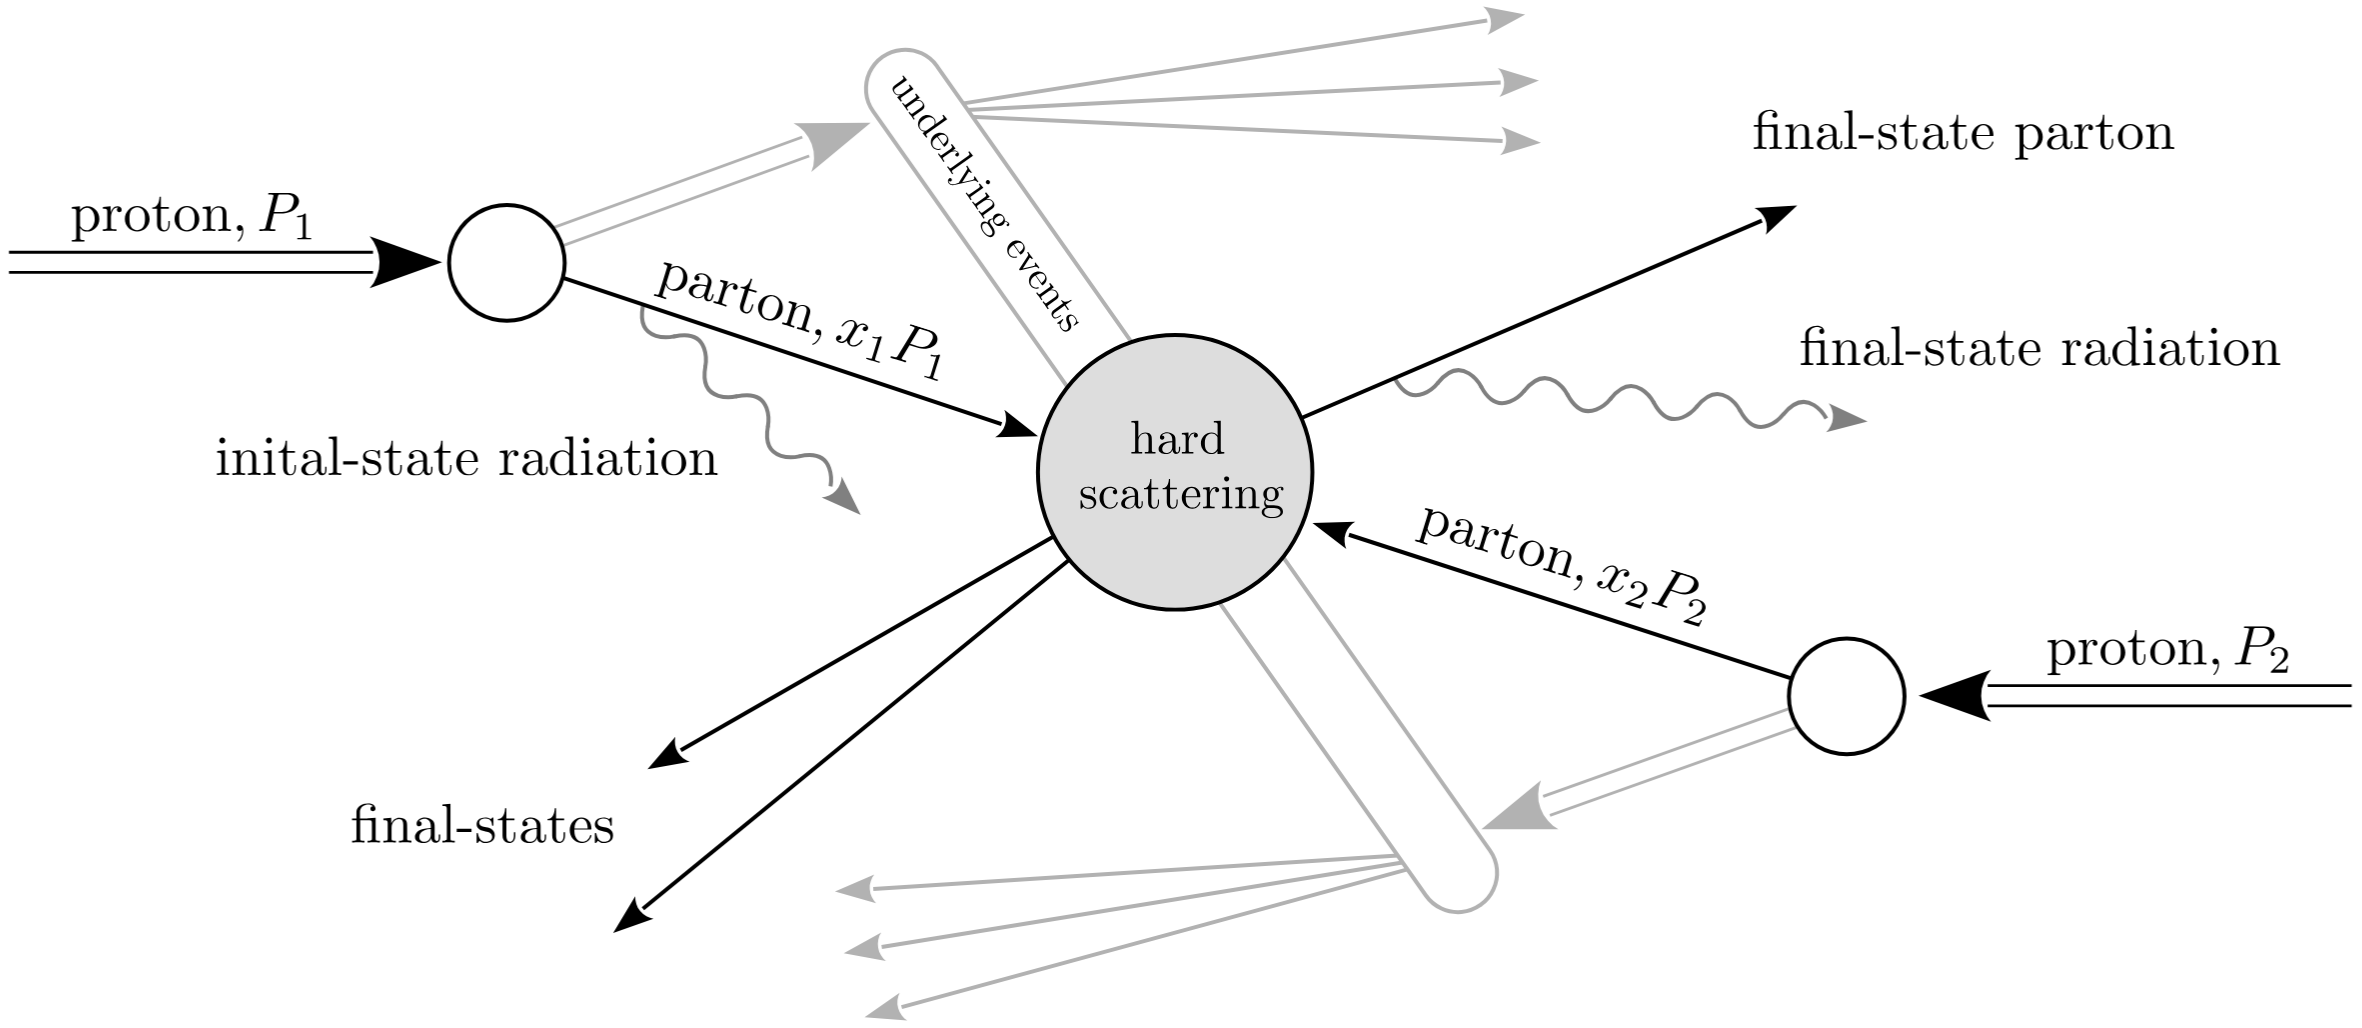
\includegraphics[width = 0.90 \textwidth]{part-scatt.png}
  \caption{Schematics of hard hadronic scattering. Due to asymptotic freedom, individual partons can be assumed to be free particles, so that their (hard) scattering can be computed via perturbative QCD. Initial- and final-state radiation accounts for beyond-leading-order effects. Figure from \cite{Asteriadis-2020}.}
  \label{fig:part-scatt}
\end{figure}

\subsection{Hadronic scattering}

Theoretical predictions for hard hadronic scattering are based on the factorization theorem \cite{Collins-1989}, which states that hadronic cross-sections can be computed from partonic cross-sections as:
\begin{equation}
  \dd\hcs_{h_1,h_2}(P_1 , P_2) = \sum_{a,b} \int_{[0,1]^2} \dd \xi_1 \dd \xi_2 \, f_a^{(h_1)}(\xi_1, \fac^2) f_b^{(h_2)}(\xi_2, \fac^2) \, \dd\pcs_{a,b}(\xi_1 P_1, \xi_2 P_2, \rc, \ren^2, \fac^2)
  \label{eq:fact-th}
\end{equation}
Here, the two scattering hadrons $ h_1 , h_2 $ have momenta $ P_1 , P_2 $, while the scattering partons $ a , b $ have momentum fractions $ \xi_1 P_1 , \xi_2 P_2 $. The factorization scale $ \fac $ is taken to be equal to the renormalization scale $ \ren $ for the rest of this work.

The link between hadron-scale physics and parton-scale physics is given by \bctxt{parton distribution functions} (PDFs): in general, $ f_a^{(h)}(\xi) $ is the numerical probability of finding a parton $ a $ inside the hadron $ h $ with a definite energy fraction $ \xi : p_a = \xi P_h $, where $ p_a $ and $ P_h $ are the momenta of the parton and of the hadron, respectively. A crucial property of PDFs is their universality, as they are energy-independent: this means that they can be measured in a particular process and then used in many others. However, they incapsulate non-perturbative effects which are poorly understood, thus they have not been computed from first principles so far.

Another instance of non-perturbative effects arises when considering that, after the partonic interaction, final-state partons can be clustered in the so-called jets: despite the difficulty in formally defining jets (for a review of various jet algorithms, see \cite{Salam-2010}), they can intuitively be pictured as seeds of hadronic energy flows which are barely affected by non-perturbative QCD effects. While on short time-scales QCD can be treated perturbatively, on long time-scales QCD partons (and so jets too) are subject to the phenomenon of \bctxt{hadronization}.

\begin{figure}
  \centering
  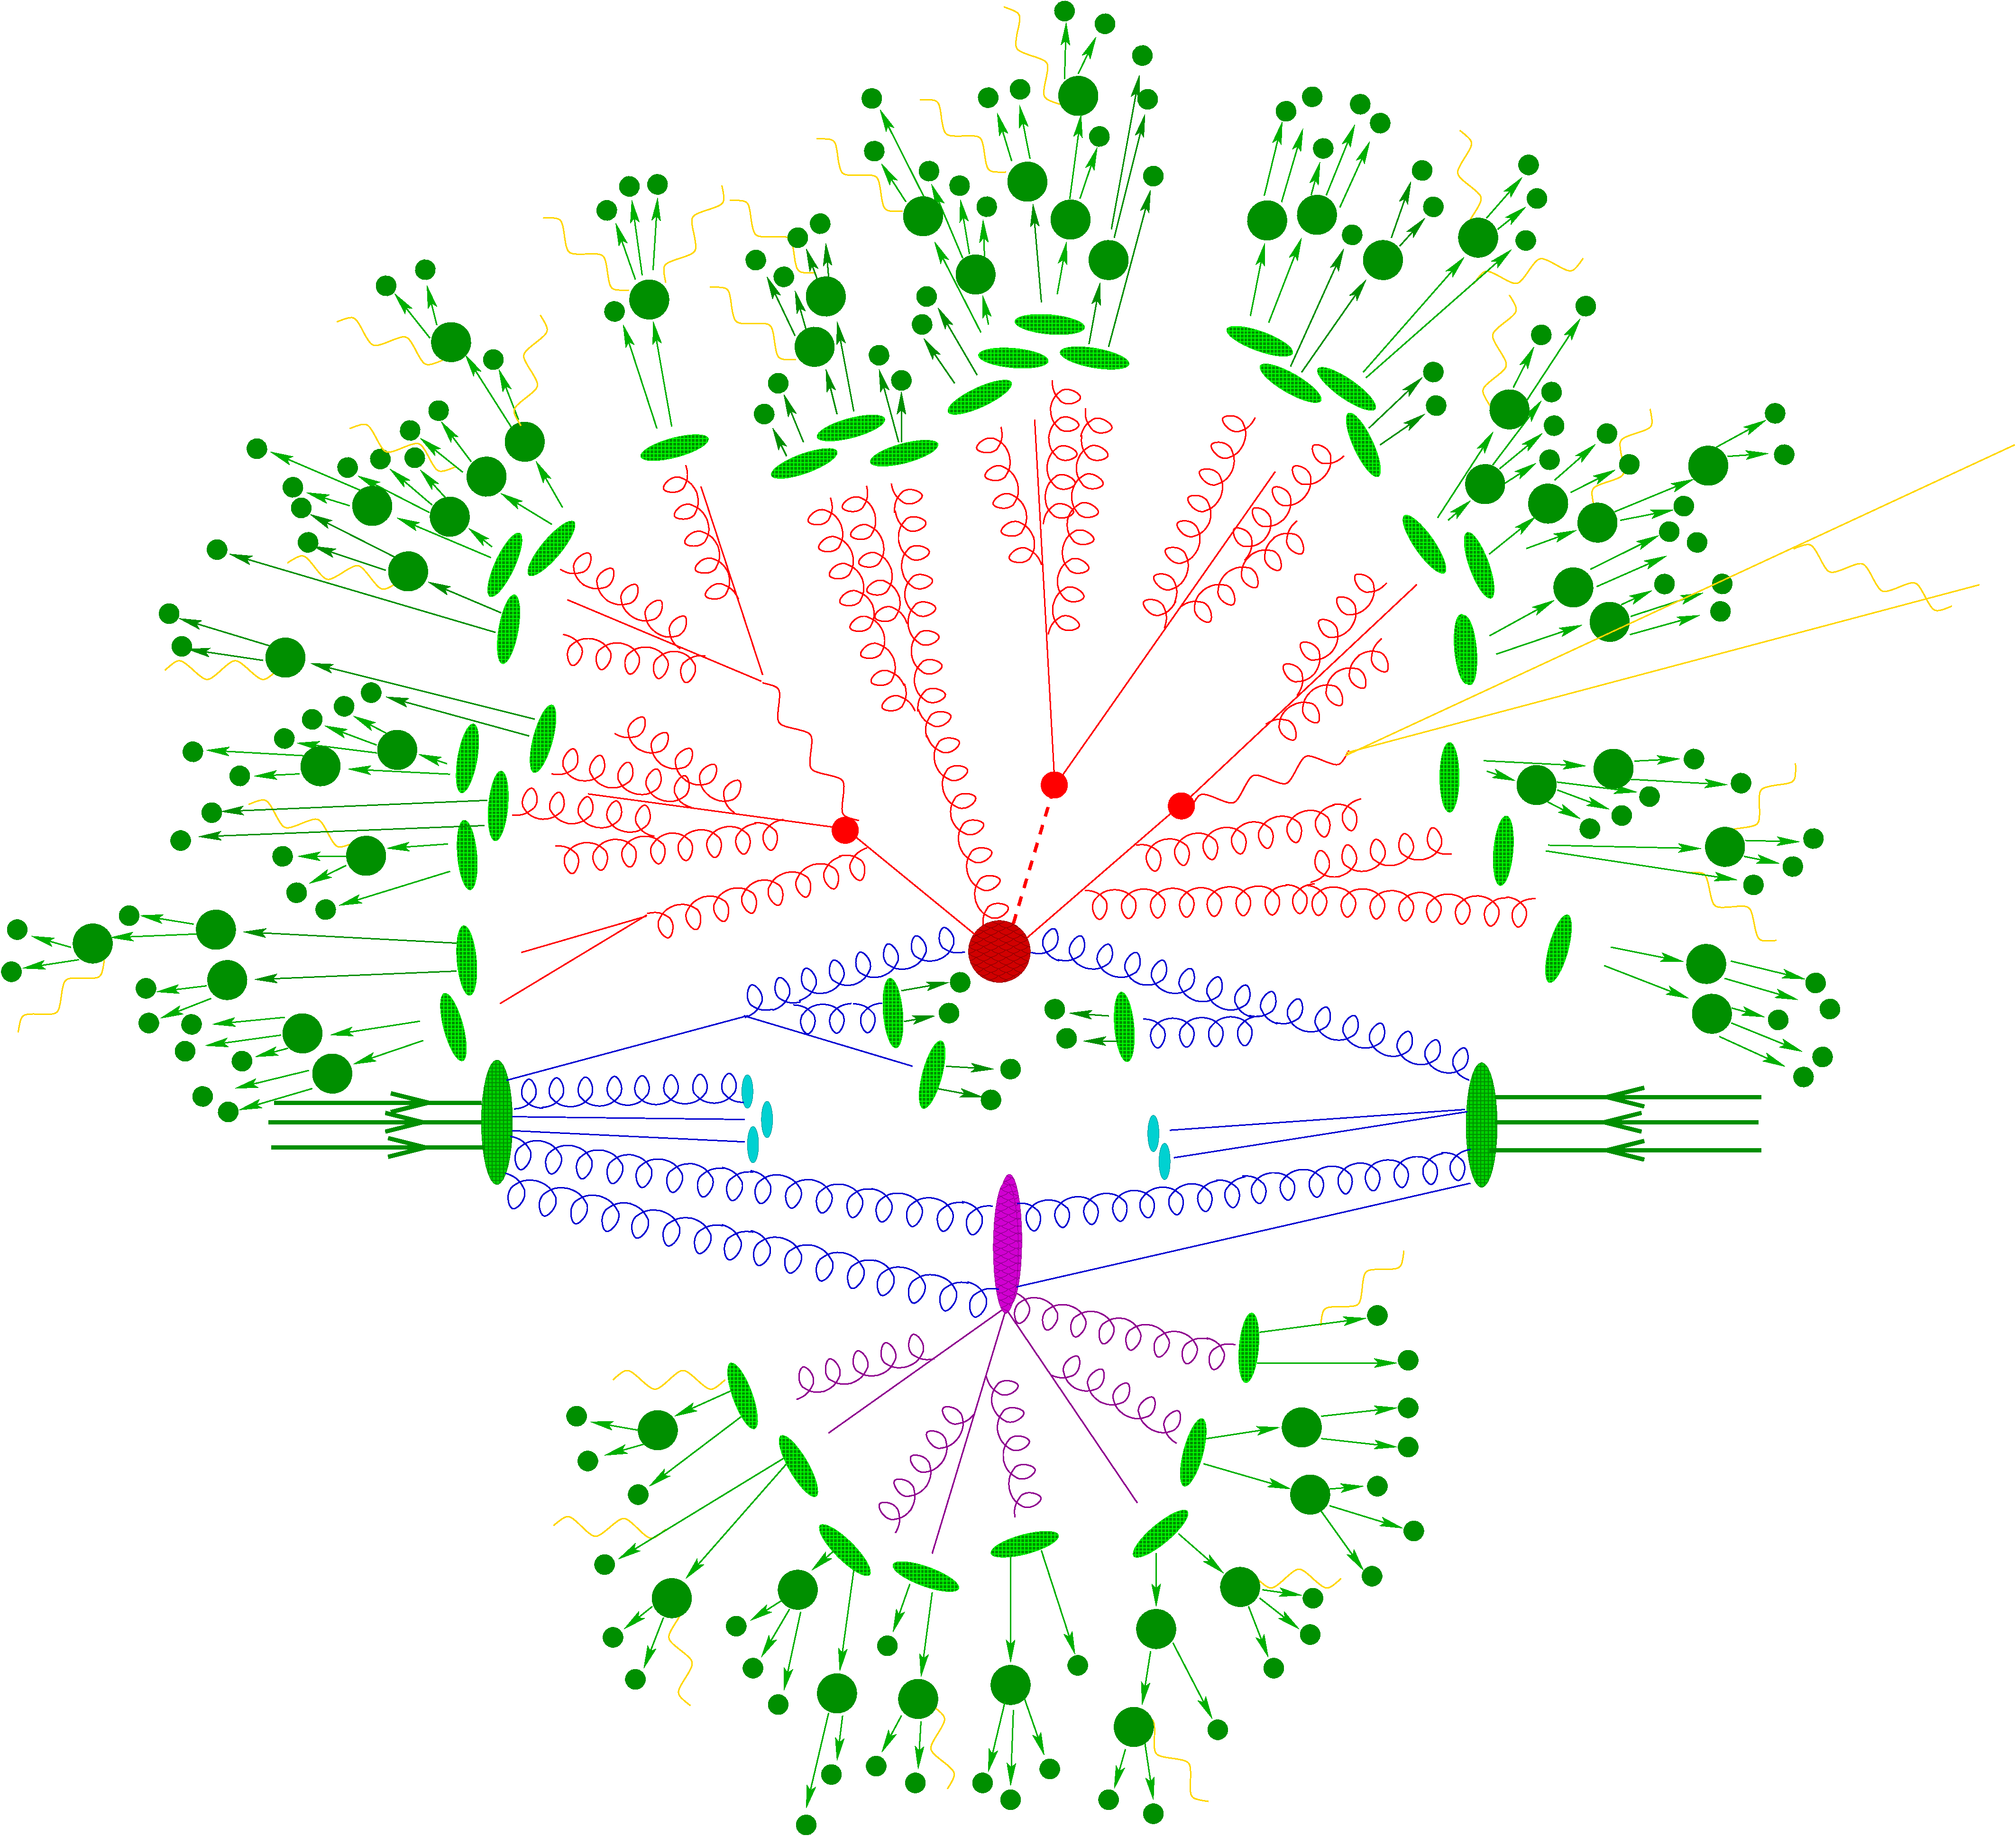
\includegraphics[width = 1.00 \textwidth]{hadr-scatt.pdf}
  \caption{Hadronization of jets produced in a hard hadronic scattering. Incoming hadrons produce initial-state radiation (blue), which determines two hard scattering events (red and purple blobs): these scatterings give rise to partonic jets (red and purple) which undergo hadronization (light green blobs), eventually decaying into heavy hadrons (dark green blobs) and soft radiation (yellow). Figure from \cite{Hoche-2014}.}
  \label{fig:hadr-scatt}
\end{figure}

Hadronization can be explained by considering a solution to \eref{eq:ren-gr}, found introducing a reference scale $ \mu $:
\begin{equation}
  \rcr = \frac{\rc(\mu^2)}{1 + 2 \rc(\mu^2) \frac{\beta_0}{4\pi} \log \frac{\ren^2}{\mu^2}}
\end{equation}
For example, $ \rc(m_Z^2) \approx 0.118 $ \cite{PDG-2024}. It is customary to introduce a QCD scale $ \qcd \approx 300 \mev $, so that:
\begin{equation}
  \rcr \equiv \frac{1}{2\frac{\beta_0}{4\pi} \log \frac{\ren^2}{\qcd^2}}
\end{equation}
This expression shows that $ \ren \gg \qcd $ is the perturbative region, where asymptotic freedom makes $ \rc $ small enough for perturbative techniques. On the other hand, for $ \ren \rightarrow \qcd $ a Landau pole is present: this pole signals the breakdown of perturbation theory and the hadronization of partons, i.e. their confinement into bound states (hadrons).

As illustrated in \figref{fig:hadr-scatt}, the hard scattering process occurs at high energy $ Q \gg \qcd $ (typically $ Q \sim 1\tev $ at the LHC), resulting in jets which are unaffected by non-perturbative QCD, as their energy is well above the QCD scale; however, this energy is radiated off in the form of parton showers, and, when the threshold energy $ \qcd $ is reached, non-perturbative effects come into play, resulting in the hadronization of jets.

\subsection{Partonic scattering}

For the rest of this work, the analysis is restricted to perturbative effects only. As the partonic scattering can be treated with perturabtion theory, the partonic cross section for the scattering of two partons $ a , b $ with momenta $ p_1 , p_2 $ can be expressed as a power series in the running coupling:
\begin{equation}
  \dd\pcs_{a,b}(p_1 , p_2) = \sum_{n \in \N_0} \dd\pcs_{a,b}^{(n)}(p_1 , p_2)
  \label{eq:part-ser-exp}
\end{equation}
where each term is $ \dd\pcs^{(n)} \sim \rc^{n_0 + n} $, with $ n_0 \in \N $ giving the dependence on $ \rcr $ due to the leading-order (LO) process, which is usually (but not always) a tree-level process.

The $ n \ge 1 $ terms form what are denoted by QCD corrections. Focusing on next-to-leading-order (NLO) corrections, they can be of two kinds: real corrections and virtual corrections. Real corrections consist in the emission of an additional parton as initial- or final-state radiation, while virtual corrections present an additional partonic loop. Examples of a real and a virtual correction to the Drell-Yan process may be:
\begin{equation*}
  \begin{tikzpicture}
    \begin{feynman}

      \vertex (a1) {\(q\)};
      \vertex[below = 3cm of a1] (a2) {\(\bar{q}\)};

      \vertex[below = 1.5cm of a1] (b1) {};
      \vertex[right = 2.25cm of b1, dot] (v1) {};

      \vertex[right = 2.25cm of v1, dot] (v2) {};
      \vertex[right = 2.25cm of v2] (b2) {};

      \vertex[above = 1.5cm of b2] (a3) {\(e^-\)};
      \vertex[below = 1.5cm of b2] (a4) {\(e^+\)};

      \vertex[dot] (c1) at ($(a1) + (1.5,-1)$) {};
      \vertex (c2) at ($(c1) + (1.5,1)$) {\(g\)};

      \diagram* {
	(a1) -- [fermion] (v1),
	(a2) -- [anti fermion] (v1),

	(v1) -- [photon, edge label = \(\gamma^*\)] (v2),

	(v2) -- [fermion] (a3),
	(v2) -- [anti fermion] (a4),

	(c1) -- [gluon] (c2),
      };
    \end{feynman}
  \end{tikzpicture}
  \qquad \qquad
  \begin{tikzpicture}
    \begin{feynman}

      \vertex (a1) {\(q\)};
      \vertex[below = 3cm of a1] (a2) {\(\bar{q}\)};

      \vertex[below = 1.5cm of a1] (b1) {};
      \vertex[right = 2.25cm of b1, dot] (v1) {};

      \vertex[right = 2.25cm of v1, dot] (v2) {};
      \vertex[right = 2.25cm of v2] (b2) {};

      \vertex[above = 1.5cm of b2] (a3) {\(e^-\)};
      \vertex[below = 1.5cm of b2] (a4) {\(e^+\)};

      \vertex[dot] (c1) at ($(a1) + (0.75,-0.5)$) {};
      \vertex[dot] (c2) at ($(a2) + (0.75,0.5)$) {};

      \diagram* {
	(a1) -- [fermion] (v1),
	(a2) -- [anti fermion] (v1),

	(v1) -- [photon, edge label = \(\gamma^*\)] (v2),

	(v2) -- [fermion] (a3),
	(v2) -- [anti fermion] (a4),

	(c1) -- [gluon, bend right, edge label' = \(g^*\)] (c2),
      };
    \end{feynman}
  \end{tikzpicture}
\end{equation*}
In general, then:
\begin{equation}
  \dd\pcs_{a,b}^{(1)}(p_1 , p_2) = \dd\pcsr_{a,b}(p_1 , p_2) + \dd\pcsv_{a,b}(p_1 , p_2) + \dd\pcspdf_{a,b}(p_1 , p_2)
\end{equation}
where $ \dd\pcsr_{a,b} $ and $ \dd\pcsv_{a,b} $ are the single-real and 1-loop corrections. The additional correction $ \dd\pcspdf_{a,b} $ is due to the collinear renormalization of PDFs.

\section{Singularities in QCD amplitudes}

The main difficulty when computing real and virtual corrections to scattering amplitudes is the presence of singularities in particular kinematic limits.

\subsection{Infrared poles}

In the case of amplitudes with real emissions, singularities arise when the energy of a gluon vanishes (\bctxt{soft singularity}) or when two massless partons are emitted in the same direction (\bctxt{collinear singularity}). To illustrate why the amplitude diverges in these limits, consider a real-emission diagram like:
\begin{equation*}
  \begin{tikzpicture}[baseline = (r.base)]
    \begin{feynman}[inline = (r.base)]
      \vertex (a);
      \vertex[right = 2.5cm of a, dot] (b) {};
      \vertex[right = 2.5cm of b, blob, minimum size = 1.2cm] (c) {};

      \vertex[above = 1.5cm of b] (d);
      \vertex[right = 1.5cm of d] (e);

      \vertex[below = 0.2em of b] (r);

      \diagram* {
	(a) -- [fermion, momentum' = \(p\)] (b),
	(b) -- [fermion, momentum' = \(p - k\)] (c),

	(b) -- [gluon, momentum = \(k\)] (e),
      };
    \end{feynman}
  \end{tikzpicture}
  \quad \sim \quad
  \frac{1}{(p - k)^2} = \frac{1}{2 E_p E_k \left( 1 - \cos \theta \right)}
\end{equation*}
where the massless approximation\footnotemark for the quark is employed. It is then clear that the amplitude diverges for $ E_k \rightarrow 0 $ and $ \theta \rightarrow 0 $ due to the propagator of the emitted virtual quark; note that quarks don't determine any soft singularities, as their energy is technically bounded from below by their mass.

\footnotetext{In the context of collider physics, light quarks are usually approximated as massless, as they have $ m_q / Q \lesssim 10^{-3} $, with $ Q \sim 1\tev $ in a typical LHC process. The only exceptions are the heavy flavours: the bottom quark is sometimes treated as massive ($ m_b \approx 4.18 \gev $), while the top quark is always treated as massive ($ m_t \approx 172 \gev $). Data from \cite{PDG-2024}.}

Both kinds of singularities in real emissions can be seen as one virtual massless parton going on-shell (in the above example, the virtual quark with momentum $ q - k $ in the massless approximantion), i.e. with $ p^2 \rightarrow 0 $: for this reason, these are called infrared (IR) singularities.

The case of virtual corrections is more complex. Indeed, virtual-correction amplitudes present an additional loop integral, which has two kinds of singularities: ultraviolent (UV) singularities and IR ones. To illustrate them, consider the following loop diagram:
\begin{equation*}
  \begin{tikzpicture}[baseline = (r.base)]
    \begin{feynman}[inline = (r.base)]

      \vertex (a) {};
      \vertex[right = 2cm of a, dot] (b) {};
      \vertex[right = 2.5cm of b, dot] (c) {};
      \vertex[right = 2cm of c, blob, minimum size = 1.2cm] (d) {};

      \vertex[below = 0.2em of a] (r) {};

      \diagram* {
	(a) -- [gluon] (b) -- [gluon, momentum' = \(p + k\)] (c) -- [gluon] (d),
	(c) -- [gluon, out = 90, in = 90, looseness = 1.5, momentum' = \(k\)] (b),
      };
    \end{feynman}
  \end{tikzpicture}
  \quad \sim \quad
  \int \frac{\dd^4k}{(2\pi)^4} \frac{1}{k^2} \frac{1}{(p + k)^2}
\end{equation*}
The UV divergence can be seen performing a Wick rotation $ k^0 \mapsto i k^0 $ and introducing a cutoff $ \Lambda $ for the Euclidean momentum's magnitude $ \abs{k_\text{E}} $: in the UV limit $ k^2 \gg p^2 $, so the integral is $ \sim \log \Lambda $, which is clearly divergent for $ \Lambda \rightarrow \infty $. However, this kind of divergences are cured through the procedure of renormalization (\secref{sec:renorm}).

IR divergences, on the other hand, arise again when virtual massless partons go on-shell, showing thus that they have the same nature as those in real corrections: in reality, Nature does not distinguish between $ \virgolette{real} $ and $ \virgolette{virtual} $ corrections, which are merely human-made categories introduce to simplify the calculations. To confirm this, while real and virtual corrections presente IR poles when considered singularly, these poles have to cancel when the two sets of corrections are added together: this is an instance of the Kinoshita--Lee--Nauenberg theorem, which asserts that the SM is IR-finite \cite{Kinoshita-1962, Lee-1964}.

% prove the general form of collinear pdf renormalization counterterms

% introduce the concept of subtraction scheme












\chapter{Preliminaries}
\selectlanguage{english}

\section{Quantum Chromodynamics}
We consider a generalized QCD with gauge group $ \SUn{n_c} $, with $ n_c $ colours and $ n = n_f + n_F $ total quark flavours ($ n_f $ massless and $ n_F $ massive quark flavours). Note that in the SM $ n_c = 3 $ and $ n = 6 $.

\subsection{Yang--Mills theories}
\label{ssec:gauge-th}

A quantum field theory can be built starting from its symmetry properties: in particular, specifying a group of local transformations, the \bctxt{gauge group}, under which the theory must be invariant. Historically, the idea of gauge theories was first explored by Yang and Mills in \cite{Yang-1954}, with the aim of studying isotopic gauge invariance for the nucleon, and then generalized by Utiyama in \cite{Utiyama-1956}. A modern treatment of gauge theories can be found in Chapter 15 of \cite{Peskin-1995}, which we follow for our discussion.

Consider $ n $ fermionic fields $ \{\psi_k(x)\}_{k = 1, \dots, n} $ and an $ n $-spinor $ \Psi(x) $ defined as:
\begin{equation}
  \Psi(x) =
  \begin{pmatrix}
    \psi_1(x) \\ \vdots \\ \psi_n(x)
  \end{pmatrix}
\end{equation}
As a gauge group, consider a $ d $-dimensional Lie group $ G $: in particular, take $ G $ to be simply-connected, so that each element can be expressed via the exponential map, and compact, so that its representations are unitary. Then, consider $ \{T^a\}_{a = 1, \dots, d} \subset \C^{n \times n} $ a representation of the associated Lie algebra $ \mathfrak{g} $, so that the action of $ G $ on $ \Psi $ can be expressed as:
\begin{equation}
  \Psi(x) \mapsto V(x) \Psi(x)
  \qquad \qquad
  V(x) \defeq \exp \left[ i \theta_a(x) T^a \right]
  \label{eq:gauge-trans}
\end{equation}
where the Lie parameters $ \{\theta_a(x)\}_{a = 1, \dots, d} \subset \mathcal{C}^\infty(\R^{1,3}) $ define a local gauge transformation. The aim is to define a Lagrangian which is invariant under this transformation, i.e. the Lagrangian of a (local) gauge theory.

Simple terms invariant under global phase rotations, like the fermion mass term $ m \bar{\Psi} \Psi $, are of course invariant under \eref{eq:gauge-trans} too, but derivatives need a careful treatment: indeed, the limit-definition of a derivative involves fields at different spacetime points, which have different transformations according to \eref{eq:gauge-trans}. In order to define a derivative of \Psi, it is necessary to introduce a factor to subtract values of $ \Psi(x) $ in a meaningful way, so consider $ \mt{U}(y,x) \in \Un{n} : \mt{U}(x,x) = 1 $ and which transforms under the action of $ G $ as:
\begin{equation}
  \mt{U}(y,x) \mapsto V(y) \mt{U}(y,x) V\dg(x)
  \label{eq:fac-cov-der}
\end{equation}
By the unitarity of the representations of $ G $, it is clear that $ \mt{U}(y,x) \Psi(x) $ and $ \Psi(y) $ have the same transformation law, so they can be meaningfully subtracted. Then, given $ n^\mu \in \R^{1,3} $, the covariant derivative of a fermionic field $ \Psi(x) $ along $ n^\mu $ is defined as:
\begin{equation}
  n^\mu D_\mu \Psi(x) \defeq \lim_{\varepsilon \rightarrow 0} \frac{1}{\varepsilon} \left[ \Psi(x + \varepsilon n) - \mt{U}(x + \varepsilon n, x) \Psi(x) \right]
  \label{eq:cov-der-def}
\end{equation}
where $ \mt{U}(y,x) $ is defined through \eref{eq:fac-cov-der}. To make this definition explicit, it is necessary to get an expression of $ \mt{U}(y,x) $ at infinitesimally-separated points. Given the unitarity of $ \mt{U}(y,x) $, it can be expressed through the generators $ \{T^a\}_{a = 1, \dots, d} $ as:
\begin{equation}
  \mt{U}(x + \varepsilon n, x) = \mt{I}_n + i g \varepsilon n^\mu A_\mu^a(x) T_a + \smo(\varepsilon^2)
  \label{eq:fac-cov-der-exp}
\end{equation}
where $ g \in \R $ is a constant. The new vector field $ A_\mu^a(x) $ (actually, $ d $ different vector fields) is a \bctxt{connection}, and it allows us to express the covariant derivative as (directly from \eref{eq:cov-der-def}):
\begin{equation}
  D_\mu = \pa_\mu - i g A_\mu^a T_a
\end{equation}
To show that $ D_\mu \Psi $ transforms in the same way as $ \Psi $, note that, from \eeref{eq:fac-cov-der}{eq:fac-cov-der-exp}:
\begin{equation*}
  \mt{I}_n + i g \varepsilon n^\mu A_\mu^a(x) T_a \mapsto I_n - \varepsilon n^\mu V(x) \pa_\mu V\dg(x) + V(x) \left( i g \varepsilon n^\mu A_\mu^a(x) T_a \right) V\dg(x) + \smo(\varepsilon^2)
\end{equation*}
Hence, the connection transforms as:
\begin{equation*}
  A_\mu^a(x) T_a \mapsto V(x) \left[ A_\mu^a(x) T_a + \frac{i}{g} \pa_\mu \right] V\dg(x) = A_\mu^a(x) T_a - f^{abc} A_\mu^a(x) \theta^b(x) T_c + \frac{1}{g} \pa_\mu \theta^a(x) T_a + \smo(\theta^2)
\end{equation*}
The second term makes it clear that the connection transforms according to the adjoint representation. From this expression, it follows that:
\begin{equation*}
  D_\mu \Psi(x) \mapsto \left[ \mt{I}_n + i \theta^a(x) T_a + \smo(\theta^2) \right] \left( \pa_\mu - i g A_\mu^a(x) T_a \right) \Psi(x) = V(x) D_\mu \Psi(x)
\end{equation*}
where the relation $ T_a T_b - i f^{abc} T_c = T_b T_a $ of the associated Lie algebra was used.

The gauge-invariant Lagrangian can thus be built using covariant derivatives (minimal coupling prescription), but one also needs to include a kinetic term for the connection, i.e. a gauge-invariant term dependent on $ A_\mu^a(x) $ only. This term can be found considering the commutator of covariant derivatives:
\begin{equation}
  [D_\mu , D_\nu] = - i g F_{\mu \nu}^a T_a
\end{equation}
with the \bctxt{field-strength tensor} defined as:
\begin{equation}
  F_{\mu \nu}^a \defeq \pa_\mu A_\nu^a - \pa_\nu A_\mu^a + g f^{abc} A_\mu^b A_\nu^c
  \label{eq:field-str}
\end{equation}
Note that the field-strength tensor is not itself a gauge-invariant quantity, as really there are $ d $ different field-strength tensors; however, it is straightforward to construct gauge-invariant combinations of $ F_{\mu \nu}^a $. In fact, in general any globally-symmetric function of $ \Psi $, $ F_{\mu \nu}^a $ and their covariant derivatives is also locally-symmetric, i.e. gauge-invariant: this follows from the construction of the covariant derivative. For a complete discussion, see Chapter 15 of \cite{Peskin-1995}.

Usually, the following gauge-invariant term is taken as kinetic term for the gauge field (i.e. the connection $ A_\mu^a(x) $):
\begin{equation}
  \tr \{(F_{\mu \nu}^a T_a)^2\} = 2 F_{\mu \nu}^a F^{\mu \nu}_a
\end{equation}
This allows defining the simplest non-Abelian gauge theory, \bctxt{Yang--Mills theory}:
\begin{equation}
  \lag_\text{YM} = - \frac{1}{4} F_{\mu \nu}^a F^{\mu \nu}_a
\end{equation}
To account for fermions interacting with the gauge field $ A_\mu^a(x) $, the Dirac Lagrangian with minimal coupling is added (see Chapter 15 of \cite{Weinberg-1996}):
\begin{equation}
  \lag = - \frac{1}{4} F_{\mu \nu}^a F^{\mu \nu}_a + \bar{\Psi} \left( i \slashed{D} - m \right) \Psi
  \label{eq:qcd-lag}
\end{equation}

\subsection{Gauge group \texorpdfstring{$ \SUn{n_c} $}{SU(n)}}
\label{ssec:sun}

The $ \SUn{n_c} $ group is the group of unitary transformations of $ n_c $-dimensional complex vectors. Its (faithful) fundamental representation thus is:
\begin{equation*}
  \SUn{n_c} = \{\mt{U} \in \C^{n_c \times n_c} : \mt{U}\mt{U}\dg = \mt{U}\dg\mt{U} = \mt{I}_{n_c} \land \det{\mt{U}} = +1 \}
\end{equation*}
The generators of $ \SUn{n_c} $ can be found setting $ \mt{U} = \exp \left( i \theta_a T^a \right) = \mt{I}_{n_c} + i \theta_a T^a + \smo(\theta^2) $ and using $ \mt{U}\dg\mt{U} = \mt{I}_{n_c} $:
\begin{equation}
  T^a = T^{a\dagger}
  \label{eq:sun-herm}
\end{equation}
Moreover, by the Jacobi formula $ (\det A(t)) \frac{\dd}{\dd t} (\det A(t)) = \tr (A(t)^{-1} \frac{\dd}{\dd t} A(t)) $ evaluated at $ t = 0 $:
\begin{equation}
  \tr T^a = 0
  \label{eq:sun-trace}
\end{equation}
The traceless condition can be generalized to all semi-simple Lie algebras.
Therefore, the generators of $ \SUn{n_c} $ are $ \C^{n_c \times n_c} $ Hermitian traceless matrices: the dimension of $ \mathfrak{su}(n_c) $ then is $ n_c^2 - 1 $.

In general, the adjoint representation of a Lie group is given by representing its generators (i.e. the basis of the Lie algebra) with the structure constants of the Lie algebra:
\begin{equation}
  (T^b_\text{ad})_{ac} \equiv \bar{T}^b_{ac} = i f^{abc}
\end{equation}
which, in the case of $ \SUn{n_c} $, are $ f^{abc} = \epsilon^{abc} $. Indeed, it can be shown by the Jacobi identity that the structure constants satisfy the Lie algebra:
\begin{equation*}
  f^{abd} f^{dce} - f^{acd} f^{dbe} = f^{bcd} f^{ade}
  \quad \iff \quad
  [[T^a,T^b],T^c] + [[T^c,T^a],T^b] + [[T^b,T^c],T^a] = 0
\end{equation*}
Moreover, since the structure constant are real, the adjoint representation is always a real representation: the adjoint representation of $ \SUn{n_c} $ has degree $ n_c^2 - 1 $.

Representation are labelled by their Casimir operators. For any simple Lie algebra, given a representation $ \mathtt{r} $, a Casimir operator is defined as:
\begin{equation}
  T^a_\mathtt{r} T^a_\mathtt{r} = C_2(\mathtt{r}) \mt{I}_{n_{\mathtt{r}}}
  \label{eq:quad-cas}
\end{equation}
This is called the \bctxt{quadratic Casimir operator}, as it is associated to $ T^2 \equiv T^a T^a $ (a Casimir operator since $ [T^b, T^2] = i f^{bac} \{T^c,T^a\} = 0 $ by antisymmetry). For the fundamental and the adjoint representations $ \mathtt{n} $ and $ \mathtt{g} $ of $ \SUn{n_c} $, the quadratic Casimir operators are (\secref{sec:cas-op}):
\begin{equation}
  \caf \equiv C_2(\mathtt{n}) = \ttr \frac{n_c^2 - 1}{n_c}
  \qquad \qquad
  \caa \equiv C_2(\mathtt{g}) = 2\ttr n_c
  \label{eq:cas-sun}
\end{equation}
where $ \ttr $ (usually taken to be $ \ttr = \frac{1}{2} $) is the trace normalization of the generators in the fundamental representation:
\begin{equation}
  \tr (T^a_\mathtt{n} T^b_\mathtt{n}) = \ttr \delta^{ab}
  \label{eq:diag-norm}
\end{equation}

\subsection{Quantization}
\label{ssec:qcd-quant}

The quantization of a non-Abelian gauge theory requires careful treatment due to the presence of spurious non-physical degrees of freedom. These can be accounted for with the Faddeev--Popov method \cite{Faddeev-1967}, i.e. imposing a gauge fixing condition and introducing non-physical ghost fields, which serve as ``negative" degrees of freedom. Then, functional quantization can be performed naturally, resulting in the following Feynman rules for the Yang--Mills Lagrangian (excluding ghost fields):
\begin{align*}
  \begin{tikzpicture}[baseline = (r.base)]
    \begin{feynman}[inline = (r.base)]
      \vertex[dot] (a) {};
      \vertex (la) at ($(a) + (-0.3,0)$) {\(a\)};
      \vertex[right = 2cm of a, dot] (b) {};
      \vertex (lb) at ($(b) + (0.3,0)$) {\(b\)};
      \vertex[below = 0.25em of b] (r);
      \diagram* {
        a -- [fermion, momentum = \(p\)] (b),
      };
    \end{feynman}
  \end{tikzpicture}
  & \quad = \quad
  \frac{i}{\slashed{p} - m} \delta_{ab}
  &
  \begin{tikzpicture}[baseline = (r.base)]
    \begin{feynman}[inline = (r.base)]
      \vertex[dot] (a) {};
      \vertex (la) at ($(a) + (-0.5,0)$) {\(\mu,a\)};
      \vertex[right = 2cm of a, dot] (b) {};
      \vertex (lb) at ($(b) + (0.5,0)$) {\(\nu,b\)};
      \vertex[below = 0.25em of b] (r);
      \diagram* {
        a -- [gluon, momentum = \(k\)] (b),
      };
    \end{feynman}
  \end{tikzpicture}
  & \quad = \quad
  \frac{-i g_{\mu \nu}}{k^2} \delta_{ab}
  \\
  \begin{tikzpicture}[baseline = (r.base)]
    \begin{feynman}[inline = (r.base)]
      \vertex (a) {};
      \vertex (la) at ($(a) + (0,0.1)$) {\(\mu,a\)};
      \vertex[dot, below = 1.5cm of a] (v) {};
      \vertex[below = 0.8cm of v] (z) {};
      \vertex[left = 1.3cm of z] (b) {};
      \vertex (lb) at ($(b) + (-0.1,0.05)$) {\(b\)};
      \vertex[right = 1.3cm of z] (c) {};
      \vertex (lc) at ($(c) + (0.1,0)$) {\(c\)};
      \vertex[below = 0.25em of v] (r);
      \diagram* {
        (a) -- [gluon] (v),
        (b) -- [fermion] (v),
        (c) -- [anti fermion] (v),
      };
    \end{feynman}
  \end{tikzpicture}
  & \quad = \quad
  i g \gamma^\mu T^a \delta_{bc}
  &
  \begin{tikzpicture}[baseline = (r.base)]
    \begin{feynman}[inline = (r.base)]
      \vertex (a) {};
      \vertex (la) at ($(a) + (0,0.1)$) {\(\mu,a\)};
      \vertex[dot, below = 1.5cm of a] (v) {};
      \vertex[below = 0.8cm of v] (z) {};
      \vertex[left = 1.3cm of z] (b) {};
      \vertex (lb) at ($(b) + (-0.23,0.05)$) {\(\nu,b\)};
      \vertex[right = 1.3cm of z] (c) {};
      \vertex (lc) at ($(c) + (0.2,0)$) {\(\rho,c\)};
      \vertex[below = 0.25em of v] (r);
      \diagram* {
        (a) -- [gluon, momentum = \(p\)] (v),
        (b) -- [gluon, momentum = \(q\)] (v),
        (c) -- [gluon, momentum = \(k\)] (v),
      };
    \end{feynman}
  \end{tikzpicture}
  & \quad = \quad
  \begin{array}{l}
    g f^{abc} \,[\, g^{\mu \nu} \left( p - q \right)^\rho \\
    \quad\,\ \ +\, g^{\nu \rho} \left( q - k \right)^\mu \\
    \quad\,\ \ +\, g^{\rho \mu} \left( k - p \right)^\nu \,]
  \end{array}
\end{align*}
\begin{equation*}
  \begin{tikzpicture}[baseline = (r.base)]
    \begin{feynman}[inline = (r.base)]
      \vertex[dot] (v) {};

      \vertex[above = 1.3cm of v] (z1) {};
      \vertex[left = 1.3cm of z1] (a) {};
      \vertex[right = 1.3cm of z1] (b) {};

      \vertex[below = 1.3cm of v] (z2) {};
      \vertex[left = 1.3cm of z2] (c) {};
      \vertex[right = 1.3cm of z2] (d) {};

      \vertex (la) at ($(a) + (-0.23,-0.05)$) {\(\mu,a\)};
      \vertex (lb) at ($(b) + (0.2,0)$) {\(\nu,b\)};
      \vertex (lc) at ($(c) + (-0.2,-0.05)$) {\(\rho,c\)};
      \vertex (ld) at ($(d) + (0.23,0)$) {\(\sigma,d\)};

      \vertex[below = 0.25em of v] (r);

      \diagram* {
        (a) -- [gluon] (v),
        (b) -- [gluon] (v),
        (c) -- [gluon] (v),
        (d) -- [gluon] (v),
      };
    \end{feynman}
  \end{tikzpicture}
  \quad = \quad
  \begin{array}{l}
    - i g^2 \,[\, f^{abe} f^{cde} \left( g^{\mu \rho} g^{\nu \sigma} - g^{\mu \sigma} g^{\nu \rho} \right) \\
    \quad\,\ +\, f^{ace} f^{bde} \left( g^{\mu \nu} g^{\rho \sigma} - g^{\mu \sigma} g^{\nu \rho} \right) \\
    \quad\,\ +\, f^{ade} f^{bce} \left( g^{\mu \nu} g^{\rho \sigma} - g^{\mu \rho} g^{\nu \sigma} \right) \,]
  \end{array}
\end{equation*}
The peculiar nature of non-Abelian gauge theories is due to the possibility for gauge bosons to self-interact (last two vertices).

In the case of QCD, the quanta of the $ n $ spinor fields are the $ n $ quark falvours, while the $ n_c^2 - 1 $ gauge fields are gluon fields, and their colour charges are given by their respective $ \SUn{n_c} $ representations: $ n_c $ charges for the quarks (fundamental $ n $-dimensional representation) and $ n_c^2 - 1 $ charges for the gluons (adjoint representation).

\section{Renormalization scheme}
\label{sec:renorm}

The computation of NLO corrections to scattering processes in a generic QFT involves UV-divergent loop amplitudes. In order to obtain finite results from these divergences, a renormalization scheme must be implemented.

The generalization of Catani's formula for IR singularities in virtual corrections is provided in \cite{Catani-2001} in a charge-unrenormalized (but mass-renormalized) way, i.e. still containing UV singularities (recall \secref{sec:sing}), thus it is necessary to carry out the renormalization procedure explicitly. To this end, we formally state the renormalization scheme adopted in this work.

\subsection{Dimensional regularization}
\label{ssec:dim-reg}

As stated above, in the evaluation of loop amplitudes, both UV- and IR-singularities are encountered. The most efficient way to simultaneously regularize both types of divergences is dimensional regularization \cite{Thooft-1972, Bollini-1972}.

In general, the dimensional regularization scheme consists in the analytic continuation of loop momenta to $ d = 4 - 2 \de $ dimensions, with $ \de \in \C : \Re\de < 0 $ for IR divergences and $ \Re\de > 0 $ for UV ones. This procedure turns loop integrals into meromorphic functions of $ \de \in \C $, allowing for the isolation of divergences as poles in $ \de $.

The dimensional regularization prescription leaves freedom in choosing the dimensionality of external momenta, as well as the number of polarizations of both external and internal particles, thus allowing for the definition of different regularization schemes. We choose to work with \bctxt{conventional dimensional regularization} (CDR), in which all momenta and polarization are analytically continued to $ d $ dimensions, as opposed to the 't Hooft--Veltman scheme (HV), in which only internal momenta and polarizations are.

When considering non-chiral gauge theories like QCD, CDR is the most natural choice, as the main difference between CDR and HV is the treatment of purely $ 4 $-dimensional objects, i.e. $ \gamma^5 $ and $ \epsilon_{\mu \nu \sigma \rho} $. In particular, in CDR both the Dirac algebra and Lorentz indices are analytically continued to $ d $ dimensions, leading to a mathematical inconsistency stemming from the fact that, when $ d \notin \N $, the following identities cannot hold simultaneously\footnotemark:
\begin{equation*}
  \{\gamma^5 , \gamma^\mu\} = 0 \quad \forall \mu = 0, 1, \dots, d-1
  \qquad \qquad
  \tr\{\gamma^5 \gamma^\mu \gamma^\nu \gamma^\rho \gamma^\sigma\} = -4 i \epsilon^{\mu \nu \rho \sigma}
\end{equation*}

\footnotetext{This inconsistency is the explicit manifestation of a more profound topological issue of analytically continuing the number of dimensions: the Levi-Civita symbol in $ d = 4 $ is linked to the Grassmann algebra $ \bigwedge(\R^{1,3}) $, and in particular to its top-form, but $ \bigwedge^k(\R^d) $ is only defined for $ d \in \N $, so the top exterior subspace $ \bigwedge^d(\R^{1,d-1}) $ is meaningless for $ d \notin \N $ and the Levi-Civita symbol cannot be analytically continued to $ d = 4 - 2 \de $ dimensions.}

The choice of CDR over HV is then clear: in QCD, the only pathological objects are encountered when considering chiral vertices (e.g. for pseudoscalar mesons) and electroweak interactions, and both can be handled via known prescriptions, e.g. the Breitenlohner-Maison/'t Hooft-Veltman (BMHV) scheme \cite{Breitenlohner-1977} or the Larin scheme \cite{Larin-1993}.

\subsection{Minimal subtraction}
\label{ssec:min-sub}

Once regularized, UV-divergences have to be removed via renormalization of fields and coupling constants. As a result of the renormalization procedure, a running coupling $ \rcr $ is introduced, and its definition in terms of the bare coupling $ \bc $ depends both on the regularization and the renormalization schemes.

In this work, we renormalize the coupling in a standard way (as in \cite{Catani-1998}) using the \bctxt{modified minimal-subtraction scheme} ($ \msb $), which directly subtracts UV-divergences from the coupling:
\begin{equation}
  \bc S_\de = \rcr \ren^{2\de} \left[ 1 - \frac{1}{2} \frac{\rcr}{2\pi} \frac{\beta_0}{\de} + \smo(\rc^2) \right]
  \label{eq:msb-def}
\end{equation}
where $ \ren $ is an arbitrary renormalization scale, $ S_\de $ is the typical phase-space volume factor in dimensional regularization:
\begin{equation}
  S_\de \equiv \left( 4\pi \right)^\de e^{-\eg \de}
\end{equation}
with $ \eg = 0.5772\dots $ the Euler-Mascheroni constant, and $ \beta_0 $ is the leading-order coefficient of the QCD $ \beta $-function \eref{eq:beta-func}:
\begin{equation}
  \beta_0 \defeq \frac{11}{6} \caa - \frac{2}{3} \ttr n_q
\end{equation}
where $ n_q $ is the number of active quark flavours at the considered energy scale. In this work $ n_q = n_f $ unless otherwise specified.

An important clarification about the dimensionality of $ \bc $ and $ \rc $ is needed, due to the presence of $ \ren^{2\de} $ in \eref{eq:msb-def}. In dimensional regularization, the action remains a dimensionless quantity\footnotemark, hence, given $ \act = \int \dd^dx \, \lag $, the QCD Lagrangian \eref{eq:qcd-lag} must have dimension $ [\lag] = d $, as $ [\dd^dx] = -d $. It is now trivial to verify the following dimensions:
\begin{equation*}
  [\Psi] = \frac{d - 1}{2}
  \qquad \qquad
  [A_\mu^a] = \frac{d - 2}{2}
  \qquad \qquad
  [g] = \frac{4 - d}{2} = \de
\end{equation*}
This shows that, in dimensional regularization, $ [\bc] = 2\de $. In order to work with dimensionless quantities, then, in \eref{eq:msb-def} we chose to extract the mass dimension from $ \rc $.

\footnotetext{Recall that, in natural units $ c = \hbar = 1 $, all dimensions can be expressed as mass dimensions, since $ [T] = [L] = [M]^{-1} $.}

When dealing with scattering processes, a fundamental quantity is the amplitude of a process. In the Schrödinger picture, given a quantum system described by a Hamiltonian $ H $ and a Hilbert space $ \hilb $, the amplitude for the process $ \ket{a} \rightarrow \ket{b} $, where $ \ket{a} , \ket{b} \in \hilb $ is defined as:
\begin{equation}
  \ampl \defeq \braket{b | \smat(t , t_0) | a}
\end{equation}
where $ \Delta t \equiv t - t_0 $ is the time elapsed in the transition and the $ S $-matrix is defined as:
\begin{equation}
  \smat(t , t_0) \defeq e^{- i H (t - t_0)}
\end{equation}
For an $ n \rightarrow m $ scattering with defined initial- and final-state momenta, the amplitude can be written in the multi-particle phase space as:
\begin{equation}
  \ampl_{n + m} \defeq \braket{\ve{p}_1, \dots, \ve{p}_n | \smat(+\infty , -\infty) | \ve{k}_1, \dots, \ve{k}_m} 
\end{equation}
where $ t, t_0 \rightarrow \pm \infty $ as to consider free-particle initial and final states (for a discussion on this adiabatic approximation, see Chapter 5 of \cite{Itzykson-1980}). The explicit expression of the amplitude can be computed from Feynman diagrams: for a complete discussion, see Chapter 4 of \cite{Peskin-1995}.

In general, we consider amplitudes $ \ampl_m $ involving $ m $ external QCD partons (gluons and quarks), with momenta $ \{p\} \equiv \{p_1, \dots, p_m\} $, and an arbitrary number of colourless particles (photons, leptons, ...). Dependence on the momenta and quantum numbers of colourless particles is always understood and not explicitly shown in this work. The $ \msb $-renormalized amplitude has the following perturbative expansion in $ \rc $:
\begin{equation}
  \ampl_m(\rcr, \ren^2 ; \{p\}) = \left( \frac{\rcr}{2\pi} \right)^q \left[ \ampl_m^{(0)}(\ren^2 ; \{p\}) + \frac{\rcr}{2\pi} \ampl_m^{(1)}(\ren^2 ; \{p\}) + \smo(\rc^2) \right]
  \label{eq:mat-exp}
\end{equation}
where the overall power is, in general, $ q \in \frac{1}{2} \N_0 $. Note that, although UV-divergences have been removed by the renormalization procedure, these amplitudes are still IR-singular as $ \de \rightarrow 0 $.

\section{Colour-space formalism}
\label{sec:colour-space}

To handle the colour structure of QCD amplitudes, we adopt the colour-space formalism as in \cite{Catani-1997}.

The $ m $ external partons in the amplitude $ \ampl_m $ each carry two indices: a colour index and a spin index. Colour indices are denoted by $ c_1, \dots, c_m $: for gluons $ c_i \equiv a_i \in \{1, \dots, n_c^2 - 1\} $, as the field-strength tensor \eref{eq:field-str} transforms according to the adjoint representation of the gauge group, while for quarks $ c_i \equiv \alpha_i \in \{1, \dots, n_c\} $, as their Dirac fields transform according to the fundamental representation of the gauge group. Spin indices, on the other hand, are denoted by $ s_1, \dots, s_m $, and they need to take into account how helicities change in CDR: for gluons $ s_i \equiv \mu_i \in \{1, \dots, d\} $, while for quarks $ s_i \in \{1,2\} $.

Consider the $ m $-parton colour-space $ \hilb_c $ and helicity-space $ \hilb_s $, and introduce an orthonormal basis in each:
\begin{equation*}
  \{\ket{c_1, \dots, c_m}\} \in \hilb_c
  \qquad \qquad
  \{\ket{s_1, \dots, s_m}\} \in \hilb_s
\end{equation*}
Note that, as these are finite-dimensional Hilbert spaces, the non-canonical (basis-dependent) isomorphisms $ \hilb_c \leftrightarrow \hilb_c^* $ and $ \hilb_s \leftrightarrow \hilb_s^* $ are well-defined\footnotemark.

\footnotetext{Given a finite-dimensional $ \K $-vector space $ V $ and a basis $ \{v_i\}_{i = 1,\dots,n} \subset V $, with $ n = \dim_\K V $, then a basis $ \{\omega^1, \dots, \omega^n\} \subset V^* $ of $ V^* \defeq \Hom(V,\K) $ is defined by $ \omega^i(v_j) = \delta^i_j $, and the function $ \varphi : V \rightarrow V^* : v_i \mapsto \omega^i $ is a \textit{non-canonical isomorphism} $ V \leftrightarrow V^* $. \\
If $ V $ is infinite-dimensional, instead, given a basis $ \{v_i\}_{i \in \mathcal{I}} \subset V $, the above construction only allows to define linearly-independent subsets of $ V^* $, which are not granted to be bases.}

Then, to make the colour-helicity structure of the $ m $-parton amplitude explicit, we define it as an abstract vector in $ \hilb_c \otimes \hilb_s $, so that:
\begin{equation}
  \ampl_m^{\{c_1, \dots, c_m\}, \{s_1, \dots, s_m\}}(\{p_1, \dots, p_m\}) \equiv \braket{\{c_1, \dots, c_m\}, \{s_1, \dots, s_m\} | \ampl_m(\{p_1, \dots, p_m\})}
\end{equation}
with:
\begin{equation*}
  \ket{\{c_1, \dots, c_m\}, \{s_1, \dots, s_m\}} \equiv \ket{c_1, \dots, c_m} \otimes \ket{s_1, \dots, s_m}
\end{equation*}
Hence, it is clear that the squared amplitude summed over colours and helicities is:
\begin{equation}
  \abs{\ampl_m}^2 = \braket{\ampl_m | \ampl_m}
\end{equation}
To represent colour interactions at QCD vertices, we associate to each parton $ i $ a colour charge $ \tco_i = \{\tcc_i^a\}_{a = 1, \dots, n_c^2 - 1} $ related to the emission of a gluon. The action of $ \tco_i $ onto $ \hilb_c $ is defined by:
\begin{equation}
  \braket{c_1, \dots, c_i, \dots, c_m | \tcc_i^a | b_1, \dots, b_i, \dots, b_m} = \delta_{c_1, b_1} \dots \tcc^a_{c_i b_i} \dots \delta_{c_m, b_m}
  \label{eq:t-act}
\end{equation}
Thus, $ \{\tcc^a_{c_i b_i}\}_{a = 1, \dots, n_c^2 - 1} $ form a vector with respect to the colour index $ a $ of the emitted gluon, and they are matrices in different representations of $ \SUn{n_c} $, depending on the parton $ i $:
\begin{itemize}
  \item if $ i $ is a gluon, then $ \tcc^a_{cb} \equiv i f^{cab} $ (adjoint representation);
  \item if $ i $ is a final-state quark, then $ \tcc^a_{\alpha \beta} \equiv t^a_{\alpha \beta} $ (fundamental representation), while if it is a final-state antiquark $ \tcc^a_{\alpha \beta} \equiv - t^a_{\alpha \beta} $ (conjugate of fundamental representation);
  \item if $ i $ is an initial-state quark, by crossing-symmetry $ \tcc^a_{\alpha \beta} \equiv - t^a_{\alpha \beta}$, while if it is an initial-state antiquark $ \tcc^a_{\alpha \beta} \equiv t^a_{\alpha \beta} $.
\end{itemize}
The algebra of these QCD colour-charge operators is easily determined. First of all, we set:
\begin{equation}
  \tco_i \cdot \tco_j \equiv \sum_{a = 1}^{n_c^2 - 1} \tcc_i^a \tcc_j^a
  \label{eq:t-dot}
\end{equation}
Then, by the action \eref{eq:t-act}, it is clear that charges associated to different partons commute, i.e.:
\begin{equation}
  \tco_i \cdot \tco_j = \tco_j \cdot \tco_i
  \qquad
  \forall i \neq j \in \{1, \dots, m\}
\end{equation}
Moreover, by \ceref{eq:quad-cas}{eq:t-dot}:
\begin{equation}
  \tco_i^2 = C_i \id_{\hilb_c}
\end{equation}
with $ C_i \equiv \caf $ if $ i $ is a quark/antiquark and $ C_i \equiv \caa $ if it is a gluon, i.e. the quadratic Casimir operators \eref{eq:cas-sun}. Finally, as each vector $ \ket{\ampl_m} $ is a colour-singlet, colour conservation implies:
\begin{equation}
  \sum_{i = 1}^{m} \tco_i \ket{\ampl_m} = 0
  \label{eq:col-cons}
\end{equation}
This allows us to partially (or fully, if $ m = 2 $ or $ m = 3 $, as in Appendix A of \cite{Catani-1997}) factorize the colour-charge algebra in terms of quadratic Casimir operators.












\chapter{NSC Subtraction Scheme}
\selectlanguage{english}

The aim of the NSC subtraction scheme (SS) is to compute integrated subtraction terms which account for QCD corrections to the inclusive\footnotemark production of jets in a hadron collider, i.e. to the process:
\begin{equation}
  p + p \rightarrow X + N \,\text{jets}
\end{equation}
Here, $ X $ is a colour-neutral system. The hadron-scale physics is known to be separated from the parton-scale physics (see Section 1.1 of \cite{Collins-2011}): this makes it possible for us to only manipulate partonic cross-sections according to \eref{eq:fact-th}, where now the sum runs over all intial-state massless partons $ a $ and $ b $ which contribute to the production of the considered final state. Moreover, for the rest of this work we set $ \ren = \fac = \mu $, where $ \mu $ is the typical energy scale of the considered process.

\footnotetext{Inclusive jet production denotes the theoretical prediction (or experimental measurement) of the cross-section for the production of jets of given kinematics, while summing/integrating over all other final-state radiation and particles.}

Denoting the partons' momenta as $ p_i \equiv \xi_i P_i $, $ i = 1,2 $, and suppressing the explicit dependence on the running coupling and the renormalization scale, it is possible to express the LO term of \eref{eq:part-ser-exp} as (see \secref{sec:ph-sp-p}):
\begin{equation}
  \dd\pcs_{a,b}^{(0)}(p_1 , p_2) \defeq \sum_\text{f} \frac{\mathcal{N}}{2\hat{s}} \int \lps_n \, \abs{\ampl^{(0)}_m(p_1, p_2, p_X, p_\text{f})}^2 \op_m(p_X, p_\text{f})
  \label{eq:ds-lo}
\end{equation}
where $ \hat{s} \equiv 2 p_1 \cdot p_2 $ is the partonic center-of-mass (CM) energy squared, $ p_\text{f} $ is the total final-state momentum and the normalization factor $ \mathcal{N} $ includes all necessary symmetry factors (e.g. $ (\ngl!)^{-1} $, with $ \ngl $ number of resolved gluons in the final state), as well as averaging factors for initial-state colours and helicities. The sum runs over all possible partonic final states for the considered process (formalized in the next section).

Note that $ \op_m $ is an IR-finite measurement function defining the observable, which ensures that the final state contains at least $ N $ resolved jets: in particular, if the energy of a final-state gluon vanishes (soft limit), or if two partons become collinear to one another (collinear limit), then $ \op_{m + n} \rightarrow \op_{m + n - 1} $ for $ n \in \N $, and $ \op_m \rightarrow 0 $.

Similarly, it is possible to write the NLO corrections in \eref{eq:part-ser-exp} as:
\begin{equation}
  \dd\pcs_{a,b}^\text{R}(p_1 , p_2) \defeq \sum_\text{f} \frac{\mathcal{N}_\text{R}}{2\hat{s}} \int \lps_{m+1} \, \abs{\ampl^{(0)}_{m+1}(p_1, p_2, p_X, p_\text{f})}^2 \op_{m+1}(p_X, p_\text{f})
  \label{eq:real-cs}
\end{equation}
\begin{equation}
  \dd\pcs_{a,b}^\text{V}(p_1 , p_2) \defeq \sum_\text{f} \frac{\mathcal{N}_\text{V}}{2\hat{s}} \int \lps_m \, 2\Re \braket{\ampl_m^{(0)} | \ampl_m^{(1)}} \op_m(p_X, p_\text{f})
  \label{eq:virt-cs}
\end{equation}
\begin{equation}
  \dd\pcs_{a,b}^\text{C}(p_1 , p_2) \defeq \frac{\rcr}{2\pi} \frac{1}{\de} \sum_c \int_0^1 \frac{\dd z}{z} \left[ \hat{P}_{c,a}^{(0)}(z) \dd\pcs_{c,b}^{(0)}(z p_1 , p_2) + \hat{P}_{c,b}^{(0)}(z) \dd\pcs_{a,c}^{(0)}(p_1 , z p_2) \right]
  \label{eq:pdf-cs}
\end{equation}
Note that in \eref{eq:real-cs} the final state contains $ m + 1 $ partons. The Altarelli-Parisi splitting kernels are listed in \secref{sec:spl-func}, and proof of \eref{eq:pdf-cs} is provided in \secref{ssec:coll-ren}.

The rest of this chapter is devoted to the extrapolation of IR-singularities from \eeref{eq:real-cs}{eq:pdf-cs}, proving their cancellation and providing the associated integrated counterterms.

\section{Nested subtraction}

As suggested by the name, in the NSC SS the IR-poles of real corrections are removed sequentially, starting from those arising from soft limits and then subtracting the collinear ones from the soft-regulated terms.

To show this procedure, we introduce some notation. First of all, we define the integrand function in \eeref{eq:ds-lo}{eq:real-cs} as:
\begin{equation}
  \flm_{a,b}[\fs{n}{m}] \equiv \nsym \abs{\ampl_m^{(0)}(p_1, p_2, p_X, p_\text{f})}^2 \op_m(p_X, p_\text{f})
\end{equation}
where $ \fs{n}{m} $ is the set of $ m $ final-state partons and $ \mathcal{N}_\text{sym} $ is the relative symmetry factor. The index $ n \in \en_m(a,b,X) $ enumerates all the possible QCD final states which may contribute to the partonic process: these include all combinations of flavours $ \{f_i\}_{i = 1,\dots,m} $ consistent with the initial state $ (a,b) $ and the color-singlet $ X $. In the following, we suppress the arguments of $ \en_m $. The integration on the $ m $-parton final-state phase space is instead defined as:
\begin{equation}
  \ips{\flm_{a,b}[\fs{n}{m}]} \defeq \navg \int \lps_m \, \flm_m^{a,b}[\fs{n}{m}]
\end{equation}
Then, we can rewrite \eeref{eq:ds-lo}{eq:real-cs} as:
\begin{equation}
  2\hat{s}\, \dd\pcs_{a,b}^{(0)} = \sum_{n \in \en_m} \ips{\flm_{a,b}[\fs{n}{m}]}
  \qquad \qquad
  2\hat{s}\, \dd\pcs_{a,b}^\text{R} = \sum_{n \in \en_{m+1}} \ips{\flm_{a,b}[\fs{n}{m+1}]}
  \label{eq:lo-real}
\end{equation}

Soft and collinear singularities are isolated through operators acting on $ \flm $ functions: $ \so_i $ denotes the limits in which the parton $ i $ becomes soft, while $ \co_{ij} $ that in which the partons $ i $ and $ j $ become collinear to each other. In particular, these operators extract only the leading aymptotic behaviour of $ \flm $ which is non-integrable in $ d = 4 $ dimensions, hence, if they act on quantities without non-integrable singularities, then they identically vanish (e.g. $ \so_i \equiv 0 $ if $ i $ is a (anti)quark).

\subsection{Partonic sets}

A delicate step is the determination of which final-state partons can become unresolved: indeed, in fixed-order perturbative QCD, the number of final-state hard partons cannot drop below the number of jets in the LO process. This means that at NLO no more than one parton can become unresolved, and this is ensured by the $ \op $ operators. In order to use symmetry arguments to minimize the number of unresolved partons that need to be considered, we can partition the set of final-state partons as:
\begin{equation*}
  \fs{n}{m} = \fsg{n}{m} \cup \fsq{n}{m} \cup \fsbq{n}{m} \cup \fsqm{n}{m} \cup \fsbqm{n}{m}
\end{equation*}
which are respectively the subsets of final-state gluons, massless quarks, massless antiquarks, massive quarks and massive antiquarks. It is also usefull to define the set of all massless partons:
\begin{equation*}
  \prt{n}{m} \equiv \{a,b\} \cup \fsg{n}{m} \cup \fsq{n}{m} \cup \fsbq{n}{m} \equiv \{a,b\} \cup \fsu{n}{m}
\end{equation*}
as we only consider massless initial-state partons. Note that $ \fsq{n}{m} $ and $ \fsbq{n}{m} $ can be further partitioned into sets of definite massless quark flavours, and the same can be done with $ \fsqm{n}{m} $ and $ \fsbqm{n}{m} $ with massive quark flavours.

For NLO real emissions we consider an additional parton, i.e. a final state $ \fs{n}{m+1} $ with $ n \in \en_{m+1} $. To extract soft singularities from \eref{eq:lo-real}, we first consider a partition of unity such that:
\begin{equation}
  \sum_{i \in \fsu{n}{m+1}} \Delta^i = 1
  \quad : \quad
  \so_i \Delta^j = \delta_i^j
  \quad \land \quad
  \co_{ij} \Delta^k =
  \begin{cases}
    0 & i,j \neq k \\
    1 & i = k \,,\, j \in \{a,b\} \\
    z_{k,j} & i = k \,,\, j \in \fsu{n}{m+1} - \{i\}
  \end{cases}
  \label{eq:delta-part}
\end{equation}
with $ z_{k,j} \equiv E_k / (E_k + E_j) $. An explicit construction of these damping factors is given in \secref{sec:unit-part}. It is clear that a term multiplied by $ \Delta^i $ vanishes if any parton other than $ i $ becomes unresolved, thus this partition allows for the extraction of single unresolved partons:
\begin{equation*}
  2\hat{s}\, \dd\pcs_{a,b}^\text{R} = \sum_{n \in \en_{m+1}} \sum_{i \in \fsu{n}{m+1}} \ips{\Delta^i \flm_{ab}[\fs{n}{m+1}]}
\end{equation*}
We can relabel the potentially-unresolved parton $ i $ in each term as $ \ur_{f_i} $: then, for each allowed massless\footnotemark flavour $ f $, there are $ N_f $ equal terms, where $ N_f $ is the number of final-state partons of flavour $ f $. We can account for the cancellation of these factors with symmetry factors defining $ \fs{n}{m}(\ur_f) \equiv \fs{n}{m+1} - \{\ur_f\} $, thus imposing that the symmetry factors of $ \flm_{a,b}[\fs{n}{m}(\ur_f)] $ are determined ignoring $ \ur_f $ (i.e. implicitly multiplying by $ N_f $), but with the convention that the amplitude in $ \flm_{a,b}[\fs{n}{m}(\ur_f)] $ still contains the potentially-unresolved parton $ \ur_f $. Therefore:
\begin{equation}
  \begin{split}
    2\hat{s}\, \dd\pcs_{a,b}^\text{R}
    & = \sum_{n \in \en_{m+1}(g)} \ips{\Delta^\ur \flm_{a,b}[\fs{n}{m}(\ur_g)]} + \sum_{\rho = 1}^{n_f} \sum_{n \in \en_{m+1}(q_\rho)} \ips{\Delta^{\ur} \flm_{a,b}[\fs{n}{m}(\ur_{q_\rho})]} \\
    & \quad\, + \sum_{\rho = 1}^{n_f} \sum_{n \in \en_{m+1}(\bar{q}_\rho)} \ips{\Delta^{\ur} \flm_{a,b}[\fs{n}{m}(\ur_{\bar{q}_\rho})]}
  \end{split}
\end{equation}
where $ \en_m(f) \subset \en_m : N_f \ge 1 $ denotes the subset of possible final states with at least one parton of flavour $ f $.

\footnotetext{Massive partons cannot go unresolved, as they do not determine neither soft nor collinear singularities.}

Now, the nested subtraction procedure introduced in \cite{rontsch-2017} can be applied. In particular, for each term we rewrite the identity operator as:
\begin{equation}
  \id = \so_\ur + \sum_{i \in \prt{n}{m}(\ur)} \oso_\ur \co_{i\ur} + \nlo^\ur
  \qquad \qquad
  \nlo^\ur \defeq \sum_{i \in \prt{n}{m}(\ur)} \oso_\ur \oco_{i\ur} \omega^{\ur i}
  \label{eq:nest-sub}
\end{equation}
where we defined the notation for generic operators $ \overline{\mathcal{O}} \equiv \id - \mathcal{O} $ and introduced an angular partition of unity (see \secref{sec:unit-part}):
\begin{equation}
  \sum_{i \in \prt{n}{m}(\ur)} \omega^{\ur i} = 1
  \quad : \quad
  \co_{j\ur} \omega^{\ur i} = \delta_j^i
  \label{eq:omega-part}
\end{equation}
There now remains to understand how the operators in \eref{eq:nest-sub} act on the $ \flm $ functions and how the a parton set $ \fs{n}{m}(\ur) $ changes when $ \ur $ effectively becomes unresolved.

\subsection{Soft limits}

\subsection{Collinear limits}

\subsubsection{Soft-collinear limits}

\subsection{Real operators}

\section{Non-real corrections}

\subsection{Virtual corrections}

\subsection{Collinear renormalization}
\label{ssec:coll-ren}

\section{Integrated counterterms}












\chapter{NSC SS with Massive Quarks}
\selectlanguage{english}

The NSC SS, as developed in \cite{rontsch-2023, rontsch-2503, rontsch-2509}, does not include the possibility of massive final-state partons. In this chapter, we prove the cancellation of poles in the case of a general final-state massive component, i.e. with $ \fsqm{n}{m} \neq \emptyset , \fsbqm{n}{m} \neq \emptyset $, and we derive the integrated counterterms in an explicit form.

The general structure of the NSC SS as illustrated in the previous chapter remains valid: in particular, massive partons do not change collinear singularities, hence the $ \ico(\de) $ operator, as well as the Mellin convolutions of generalized splitting functions, remain unchanged. The only operators that do change are $ \iso(\de) $ and $ \ivo(\de) $.

\section{Generalized operators}

\subsection{Generalized soft operator}

\eref{eq:soft-lim} holds in general, thus to generalize the soft operator we only have to compute integrated eikonal factors in the case of massive partons. To do so, we choose a different parametrization of the phase space of the parton $ \ur_g $:
\begin{equation}
  \dd^{d-1} p = \dd p_1 \, \dd p_2 \, \dd^{d-3} p_\perp = \dd p_1 \, \dd p_2 \, \dd p_\perp \, p_\perp^{d-4} \dd \Omega_{d-4}
\end{equation}
Then, we perform a transformation to polar coordinate $ (p_1 , p_2 , p_\perp) \mapsto (p_0 , \vartheta , \varphi) $ such that:
\begin{equation}
  p_1 = p_0 \cos \vartheta
  \qquad \qquad
  p_2 = p_0 \sin \vartheta \cos \varphi
  \qquad \qquad
  p_\perp = p_0 \sin \vartheta \sin \varphi
\end{equation}
The condition $ p_\perp \in \R^+_0 $ implies $ \varphi \in [0,\pi] $, while $ \vartheta \in [0,\pi] $ by definition. As $ p_0 = E $ for gluons, the phase-space measure becomes:
\begin{equation}
  [\dd p] \equiv \frac{\dd^{3-2\de}p}{(2\pi)^{3-2\de}2E} \theta(\ema - E) = \frac{\dd \Omega_{-2\de}}{2(2\pi)^{3-2\de}} \dd E\, E^{1-2\de} \theta(\ema - E) \dd \cos \vartheta \dd \varphi \left( \sin \vartheta \sin \varphi \right)^{-2\de}
\end{equation}
Now we can perform the integration of the eikonal factor $ \eik_{i,j} $:
\begin{equation*}
  \begin{split}
    \int [\dd p_\ur] \eik_{i,j}
    & = \int_{\mathbb{S}^{-2\de}} \frac{\dd \Omega_{-2\de}}{2(2\pi)^{3-2\de}} \int_0^{\ema} \frac{\dd E_\ur}{E_\ur^{1-2\de}} \int_{-1}^1 \dd \cos \vartheta \int_0^\pi \dd \varphi \left( \sin \vartheta \sin \varphi \right)^{-2\de} \frac{\mm{p}_i \cdot \mm{p}_j}{(\mm{p}_i \cdot \mm{p}_\ur) (\mm{p}_j \cdot \mm{p}_\ur)} \\
    & = - \frac{2^{1-2\de} \pi^{-\de}}{2(2\pi)^{3-2\de}} \frac{\Gamma(1-\de)}{\Gamma(1-2\de)} \frac{\ema^{-2\de}}{2\de} \pi \eit_{i,j} = - \frac{1}{\de} \frac{\pi^\de}{16\pi^2} \frac{\Gamma(1-\de)}{\Gamma(1-2\de)} \ema^{-2\de} \eit_{i,j}(\de)
  \end{split}
\end{equation*}
where we used the following identity:
\begin{equation}
  \int_{\mathbb{S}^{d-1}} \dd \Omega_{d-1} = \frac{2 \pi^{\frac{d}{2}}}{\Gamma(\frac{d}{2})} = 2^d \pi^{\frac{d}{2} - \frac{1}{2}} \frac{\Gamma\left( \frac{d+1}{2} \right)}{\Gamma(d)}
\end{equation}
and defined the generalized angular integral:
\begin{equation}
  \eit_{i,j} \equiv \frac{1}{\pi} \int_{-1}^1 \dd \cos \vartheta \int_0^\pi \dd \varphi \left( \sin \vartheta \sin \varphi \right)^{-2\de} \frac{\mm{p}_i \cdot \mm{p}_j}{(\mm{p}_i \cdot \mm{p}_\ur) (\mm{p}_j \cdot \mm{p}_\ur)}
  \label{eq:gen-int}
\end{equation}
with $ \mm{p}_i : p_i^\mu = E_i \mm{p}_i^\mu $. There only remains to evaluate $ \eit_{i,j}(\de) $ in the three possible cases for $ i $ and $ j $: massive--massive, massive--massless (note that $ \eit_{i,j}(\de) = \eit_{j,i}(\de) $) and massless--massless. The former two cases are known in the literature, e.g. Appendix D.2 of \cite{Behring-2020}, and are reported in \secref{sec:mass-int}.

To determine $ \eit_{i,j}(\de) $ in the massless--massless case, we just have to compare the expression for the integrated eikonal factor computer in \secref{ssec:soft-massless} with the above-found expression:
\begin{equation*}
  \frac{\ema^{-2\de}}{\de^2} \eta_{ij} \frac{\pi^\de}{8\pi^2} \frac{\Gamma(1-\de)}{\Gamma(1-2\de)} \,\hyp(1,1,1-\de,1-\eta_{ij}) = - \frac{1}{\de} \frac{\pi^\de}{16\pi^2} \frac{\Gamma(1-\de)}{\Gamma(1-2\de)} \ema^{-2\de} \eit_{i,j}(\de)
\end{equation*}
hence, with an abuse of notation from \secref{sec:mass-int}:
\begin{equation}
  \eitt{i,j}{-1} = - 2 \eta_{ij} \,\hyp(1,1,1-\de,1-\eta_{ij})
  \qquad
  \eitt{i,j}{k} = 0 \,\,\forall k \in \N_0
  \label{eq:i-nmnm}
\end{equation}
Inserting everything in \eref{eq:soft-lim}, we get:
\begin{equation}
  \sum_{n \in \en_{m+1}(g)} \ips{\so_\ur \Delta^\ur \flm_{a,b}[\fs{n}{m}(\ur_g)]} = [\rc] \ips{\iso(\de) \flm_{a,b}[\fs{n}{m}]}
\end{equation}
with the generalized soft operator:
\begin{equation}
  \iso(\de) \defeq \frac{1}{2\de} \left( \frac{2\ema}{\mu} \right)^{-2\de} \frac{\Gamma^2(1-\de)}{\Gamma(1-2\de)} \sum_{i,j \in \fsp{n}{m}} (\cc) \eit_{i,j}(\de)
\end{equation}

\subsection{Generalized virtual operator}

Catani's $ \ioo(\de) $ is generlized in \cite{Catani-2001}. However, as already stated, this operator is stated in a charge-unrenormalized way, hence we have to perform the renormalization of the results of this paper. In the following, we will denote charge-unrenormalized amplitudes as $ \mat $ and charge-renormalized amplitudes as $ \ampl $.

Loop corrections to the LO amplitude can be written as:
\begin{equation}
  \mat_m = \left( \frac{\bc}{4\pi \mu^{2\de}} \right)^q \left[ \mat_m^{(0)} + \frac{\bc}{4\pi \mu^{2\de}} \mat^{(1)} + \smo(\bc^2) \right]
  \label{eq:ampl-non-ren}
\end{equation}
where $ q \in \frac{1}{2} \N_0 $. Note that this equation fixes the normalization of the charge-unrenormalized amplitudes. Catani's formula reads:
\begin{equation}
  \mat_m^{(1)} = \irs(\de) \mat_m^{(0)} + \mat_m^\text{fin}
  \label{eq:gen-cat-form}
\end{equation}
where $ \mat_m^\text{fin} $ is the non-singular part of the 1-loop amplitude and Catani's operator\footnotemark is define as (in CDR):
\begin{equation}
  \irs(\de) \defeq \frac{(4\pi)^\de}{\Gamma(1-\de)} \left[ q \frac{\beta_0}{\de} + \ioo(\de) \right]
\end{equation}
\begin{equation}
  \ioo(\de) \defeq \sum_{i \neq j \in \fsp{n}{m}} (\cc) \left( \frac{\mu^2}{\abs{s_{ij}}} \right)^\de \left[ \ns_{i,j}(\de) + \frac{1}{v_{ij}} \left( \frac{i\pi}{\de} - \frac{\pi^2}{2} \right) \theta(s_{ij}) \right] - \sum_{i \in \fsp{n}{m}} \Gamma_i(\de)
  \label{eq:gen-cat}
\end{equation}
where $ v_{ij} $ is defined in \eref{eq:v-def}, $ s_{ij} \equiv 2 p_i \cdot p_j $ and the singular functions are defined in \secref{sec:cat-fun}. Inserting \eeref{eq:gen-cat-form}{eq:gen-cat} into \eref{eq:ampl-non-ren}:
\begin{multline*}
  \mat_m = \left( \frac{\bc}{4\pi \mu^{2\de}} \right)^q \bigg[ \left( 1 + \frac{(4\pi)^\de}{\Gamma(1-\de)} \frac{\bc}{4\pi \mu^{2\de}} q \frac{\beta_0}{\de} \right) \mat_m^{(0)} \\
  + \frac{(4\pi)^\de}{\Gamma(1-\de)} \frac{\bc}{4\pi \mu^{2\de}} \left( \ioo(\de) \mat_m^{(0)} + \mat_m^\text{fin} \right) + \smo(\bc^2) \bigg]
\end{multline*}
Renormalization in the $ \msb $ scheme is performed via \eref{eq:msb-def}. Substituting this to $ \bc $ yields:
\begin{equation*}
  \begin{split}
    \mat_m
    & = \left( \frac{\rc}{4\pi S_\de} \right)^q \left[ 1 - \frac{1}{2} \frac{\rc}{2\pi} \frac{\beta_0}{\de} + \smo(\rc^2) \right]^q \times \\
    & \qquad \quad \times \left[ \left( 1 + \frac{(4\pi)^\de}{\Gamma(1-\de)} \frac{\rc}{4\pi S_\de} q \frac{\beta_0}{\de} \right) \mat_m^{(0)} + \frac{(4\pi)^\de}{\Gamma(1-\de)} \frac{\rc}{4\pi S_\de} \left( \ioo(\de) \mat_m^{(0)} + \mat_m^\text{fin} \right) + \smo(\bc^2) \right] \\
    & = \left( \frac{\rc}{4\pi S_\de} \right)^q \bigg[ \left( 1 - \frac{\rc}{4\pi} q \frac{\beta_0}{\de} \left( 1 - \frac{e^{\eg\de}}{\Gamma(1-\de)} \right) \right) \mat_m^{(0)} + \\
    & \qquad \qquad \qquad \qquad \qquad \qquad \qquad \qquad \qquad \quad + \frac{e^{\eg\de}}{\Gamma(1-\de)} \frac{\rc}{4\pi} \left( \ioo(\de) \mat_m^{(0)} + \mat_m^\text{fin} \right) + \smo(\rc^2) \bigg] \\
    & = \left( \frac{\rc}{4\pi S_\de} \right)^q \left[ \mat_m^{(0)} + \frac{e^{\eg\de}}{\Gamma(1-\de)} \frac{\rc}{4\pi} \left( \ioo(\de) \mat_m^{(0)} + \mat_m^\text{fin} \right) + \smo(\de) + \smo(\rc^2) \right]
  \end{split}
\end{equation*}
Hence, we can write the renormalized relation:
\begin{equation}
  \ampl_m = \left( \frac{\rc}{2\pi} \right)^q \left[ \ampl_m^{(0)} + \frac{\rc}{2\pi} \ampl_m^{(1)} + \smo(\rc^2) \right]
\end{equation}
with:
\begin{equation}
  \ampl_m \equiv \mat_m
  \qquad \qquad
  \ampl_m^{(0)} \equiv (2S_\de)^{-q} \mat_m^{(0)}
  \qquad \qquad
  \ampl_m^\text{fin} \equiv (2S_\de)^{-q} \mat_m^\text{fin}
\end{equation}
\begin{equation}
  \ampl_m^{(1)} = \frac{1}{2} \frac{e^{\eg\de}}{\Gamma(1-\de)} \left[ \ioo(\de) \ampl_m^{(0)} + \ampl_m^\text{fin} \right]
\end{equation}
It is then clear, from \eref{eq:virt-cs}, that:
\begin{equation}
  2\hat{s}\, \dd\pcs_{a,b}^\text{V} = [\rc] \sum_{n \in \en_m} \ips{\ivo(\de) \flm_{a,b}[\fs{n}{m}]} + \sum_{n \in \en_m} \ips{\flm_{a,b}^\text{fin}[\fs{n}{m}]}
\end{equation}
where the generalized virtual operator is:
\begin{equation}
  \ivo(\de) \defeq \Re \ioo(\de) = \sum_{i \neq j \in \fsp{n}{m}} (\cc) \left( \frac{\mu^2}{\abs{s_{ij}}} \right)^\de \left[ \ns_{i,j}(\de) - \frac{1}{v_{ij}} \frac{\pi^2}{2} \theta(s_{ij}) \right] - \sum_{i \in \fsp{n}{m}} \Gamma_i(\de)
\end{equation}

\footnotetext{Note that the notation is slightly different from \cite{Catani-2001}.}

\section{Integrated counterterms}
\label{sec:int-count}

Now, there only remains to show that $ \ito(\de) $ is $ \de $-finite and find its $ \smo(\de^0) $ term $ \ito^{(0)} $. First, we show the cancellation of colour-correlated terms between the soft and virtual operators:
\begin{equation*}
  \begin{split}
    \isvo(\de)
    & = \sum_{i \neq j \in \fsp{n}{m}} (\cc) \bigg[ \frac{1}{2\de} \left( 1 - 2\lmx \de + \left( 2\lmx^2 - \frac{\pi^2}{6} \right) \de^2 + \smo(\de^3) \right) \eit_{i,j}(\de) \,+ \\
    & \quad + \left( 1 + \de \log \frac{\mu^2}{\abs{s_{ij}}} + \frac{1}{2} \de^2 \log^2 \frac{\mu^2}{\abs{s_{ij}}} + \smo(\de^3) \right) \left( \ns_{ij}(\de) - \frac{1}{v_{ij}} \frac{\pi^2}{2} \theta(s_{ij}) \right) \bigg] + \\
    & \quad + \sum_{i \in \fsp{n}{m}} \bigg[ \tco_i^2 \frac{1}{2\de} \left( 1 - 2\lmx \de + \smo(\de^2) \right) \eit_{i,i}(\de) - \Gamma_i(\de) \bigg] \\
    & = \sum_{i \neq j \in \fsp{n}{m}} (\cc) \bigg[ \left( \frac{1}{2\de} - \lmx + \left( \lmx^2 - \frac{\pi^2}{12} \right) \de \right) \left( \frac{\eitt{i,j}{-1}}{\de} + \eitt{i,j}{0} + \de \eitt{i,j}{1} \right) + \smo(\de) \\
    & \quad + \left( 1 + \de \log \frac{\mu^2}{\abs{s_{ij}}} + \frac{1}{2} \de^2 \log^2 \frac{\mu^2}{\abs{s_{ij}}} \right) \left( \frac{\nss{i,j}{-2}}{\de^2} + \frac{\nss{i,j}{-1}}{\de} + \nss{i,j}{0} - \frac{1}{v_{ij}} \frac{\pi^2}{2} \theta(s_{ij}) \right) + \smo(\de) \,+ \\
    & + \sum_{i \in \fsm{n}{m}} \left[ \tco_i^2 \left( \frac{1}{2\de} - \lmx \right) \left( \eitt{i,i}{0} + \de \eitt{i,i}{1} \right) - \Gamma_i(\de) \right] - \sum_{i \in \prt{n}{m}} \Gamma_i(\de) + \smo(\de^2)
  \end{split}
\end{equation*}
where we set $ \fsm{n}{m} \equiv \fsqm{n}{m} \cup \fsbqm{n}{m} $. To better understand the calculation, we consider each summation separately. The colour-correlated term can be written as:
\begin{multline*}
  \underbrace{\frac{1}{\de^2} \left( \frac{1}{2} \eitt{i,j}{-1} + \nss{i,j}{-2} \right) + \frac{1}{\de} \left( \frac{1}{2} \eitt{i,j}{0} + \nss{i,j}{-1} - \lmx \eitt{i,j}{-1} + \nss{i,j}{-2} \log \frac{\mu^2}{\abs{s_{ij}}} \right)}_{\ci{i,j}} + \,\smo(\de) \,+ \\
  + \underbrace{\frac{1}{2} \eitt{i,j}{1} - \lmx \eitt{i,j}{0} + \left( \lmx^2 - \frac{\pi^2}{12} \right) \eitt{i,j}{-1} + \nss{i,j}{0} - \frac{1}{v_{ij}} \frac{\pi^2}{2} \theta(s_{ij}) + \nss{i,j}{-1} \log \frac{\mu^2}{\abs{s_{ij}}} + \frac{1}{2} \nss{i,j}{-2} \log^2 \frac{\mu^2}{\abs{s_{ij}}}}_{\finc{i,j}}
\end{multline*}
where $ \ci{i,j} $ contains the $ \de $-poles and $ \finc{i,j} $ is $ \de $-finite (more precisely, $ \finc{i,j} \sim \smo(\de^0) $). The explicit expression of $ \ci{i,j} $ is derived in \secref{sec:poles}. The second summation instead reads, using \ceref{eq:i-self}{eq:g-qm}:
\begin{equation*}
  \sum_{i \in \fsm{n}{m}} \left[ \caf \left( \frac{1}{\de} - \frac{1}{\kappa_i} \log \frac{1 - \kappa_i}{1 + \kappa_i} - 2 \lmx \right) - \caf \left( \frac{1}{\de} + \frac{1}{2} \log \frac{m_{\mq_i}^2}{\mu^2} - 2 \right) \right] \equiv \sum_{i \in \fsm{n}{m}} \finm{i}
\end{equation*}
which is manifestly $ \de $-finite. Finally, from \eeref{eq:g-g}{eq:g-q}, the last summation expands as:
\begin{equation*}
  \sum_{i \in \prt{n}{m}} \Gamma_i(\de) = \sum_{i \in \prt{n}{m}} \left( \frac{1}{\de} \gamma_i + \fing{i} \right)
\end{equation*}
where we have defined the $ \smo(\de^0) $ term as:
\begin{equation}
  \fing{g} \equiv - \frac{2}{3} \ttr \sum_{\rho = 1}^{n_F} \log \frac{m_{\mq_\rho}^2}{\mu^2}
  \qquad \qquad
  \fing{q} \equiv 0
\end{equation}
We can put all the above expressions together, yielding:
\begin{equation}
    \isvo(\de) = \sum_{i \neq j \in \fsp{n}{m}} (\cc) \left[ \ci{i,j} + \finc{i,j} \right] + \sum_{i \in \fsm{n}{m}} \finm{i} - \sum_{i \in \prt{n}{m}} \left( \frac{1}{\de} \gamma_i + \fing{i} \right)
\end{equation}
We now focus on the colour-correlated term, writing $ \fsp{n}{m} \times \fsp{n}{m} = (\prt{n}{m} \cup \fsm{n}{m}) \times (\prt{n}{m} \cup \fsm{n}{m}) $:
\begin{equation*}
  \sum_{i \neq j \in \fsp{n}{m}} (\cc) \ci{i,j} = \bigg[ \sum_{i \neq j \in \prt{n}{m}} + \sum_{i \neq j \in \fsm{n}{m}} + \sum_{i \in \prt{n}{m} \,,\, j \in \fsm{n}{m}} + \sum_{i \in \fsm{n}{m} \,,\, j \in \prt{n}{m}} \bigg] (\cc) \ci{i,j}
\end{equation*}
From \secref{sec:poles}, $ \ci{i,j} $ cotributes with a $ \leg_i / \de $ term for each massless index, hence:
\begin{equation*}
  \begin{split}
    \sum_{i \neq j \in \fsp{n}{m}} (\cc) \ci{i,j}
    & = \sum_{i \neq j \in \prt{n}{m}} (\cc) \left[ \frac{\leg_i + \leg_j}{\de} + \finci{i,j} + \smo(\de) \right] \\
    & \qquad \qquad \qquad \qquad + \sum_{i \in \prt{n}{m} \,,\, j \in \fsm{n}{m}} (\cc) \frac{\leg_i}{\de} + \sum_{i \in \fsm{n}{m} \,,\, j \in \prt{n}{m}} (\cc) \frac{\leg_j}{\de} \\
    & = \sum_{i , j \in \prt{n}{m}} (\cc) \left[ \frac{\leg_i + \leg_j}{\de} + \finci{i,j} \right] - \sum_{i \in \prt{n}{m}} \tco_i^2 \left[ \frac{2\leg_i}{\de} + \finci{i,i} \right] + \smo(\de) \\
    & \qquad \qquad \qquad \qquad + \sum_{i \in \prt{n}{m} \,,\, j \in \fsm{n}{m}} (\cc) \frac{\leg_i}{\de} + \sum_{i \in \fsm{n}{m} \,,\, j \in \prt{n}{m}} (\cc) \frac{\leg_j}{\de} \\
    & = \sum_{i \in \prt{n}{m}} \frac{\leg_i}{\de} \tco_i \cdot \sum_{j \in \fsp{n}{m}} \tco_j + \sum_{i \in \fsp{n}{m}} \tco_i \cdot \sum_{j \in \prt{n}{m}} \tco_j \frac{\leg_j}{\de} - \sum_{i \in \prt{n}{m}} \tco_i^2 \frac{2\leg_i}{\de} \\
    & \qquad \qquad \qquad \qquad \qquad \qquad \qquad \qquad \qquad \qquad \quad + \sum_{i \neq j \in \prt{n}{m}} \finci{i,j} + \smo(\de) \\
    & = - \sum_{i \in \prt{n}{m}} \tco_i^2 \frac{2\leg_i}{\de} + \sum_{i \neq j \in \prt{n}{m}} \finci{i,j} + \smo(\de)
  \end{split}
\end{equation*}
where we used the colour-conservation condition \eref{eq:col-cons}. Finally, we find an expression for the sum of soft and virtual operators without colour-correlated poles:
\begin{equation}
  \isvo(\de) = - \frac{1}{\de} \sum_{i \in \prt{n}{m}} \left( \gamma_i + 2 \tco_i^2 \leg_i \right) + \isvo^{(0)} + \smo(\de)
  \label{eq:isvo}
\end{equation}
where the $ \smo(\de^0) $ term reads:
\begin{equation}
  \isvo^{(0)} \equiv \sum_{i \neq j \in \fsp{n}{m}} (\cc) \left[ \finci{i,j} + \finc{i,j} \right] + \sum_{i \in \fsm{n}{m}} \finm{i} - \sum_{i \in \prt{n}{m}} \fing{i}
  \label{eq:isvo-zero}
\end{equation}
The poles in \eref{eq:isvo} clearly cancel those in the collinear operator \eref{eq:ic-exp}, as it remains unchanged when including massive final-state partons: we only need to determine its Laurent series at $ \smo(\de) $. First, consider the generalized initial-state anomalous dimension \eref{eq:in-gen-an-dim}:
\begin{equation}
  \Gamma_{a , f_a} = \gamma_a + 2 \tco_a^2 \leg_a - \de \left[ 2 \ler_a \left( \gamma_a + 2 \tco_a^2 \leg_a \right) + 2 \tco_a^2 \leg_a^2 \right] + \smo(\de^2)
\end{equation}
Then, the generalized final-state anomalous dimension \ceref{eq:fin-gen-an-dim-pd}{eq:fin-gen-an-dim}:
\begin{equation}
  \Gamma_{i , q} = \gamma_q + 2 \caf \leg_i - \de \left[ 2 \ler_i \left( \gamma_q + 2 \caf \leg_i \right) + 2 \caf \leg_i^2 - \frac{\caf}{6} \left( 39 - 4\pi^2 \right) \right] + \smo(\de^2)
\end{equation}
\begin{equation}
  \Gamma_{i , g} = \gamma_g + 2 \caa \leg_i - \de \left[ 2 \ler_i \left( \gamma_g + 2 \caa \leg_i \right) + 2 \caa \leg_i^2 - \frac{\caa}{9} \left( 67 - 6\pi^2 \right) + \frac{23}{9} \ttr n_f \right] + \smo(\de^2)
\end{equation}
Therefore, the Laurent series of the collinear operator is:
\begin{equation}
  \ico(\de) = \frac{1}{\de} \sum_{i \in \prt{n}{m}} \left( \gamma_i + 2 \tco_i^2 \leg_i \right) + \ico^{(0)}
\end{equation}
where the $ \smo(\de^0) $ term reads:
\begin{multline}
  \ico^{(0)} = - \sum_{i \in \prt{n}{m}} \left[ 2 \ler_i \left( \gamma_i + 2 \tco_i^2 \leg_i \right) + 2 \tco_i^2 \leg_i^2 \right] + \\
  + \left( N_q + N_{\bar{q}} \right) \frac{\caf}{6} \left( 39 - 4\pi^2 \right) + N_g \left[ \frac{\caa}{9} \left( 67 - 6\pi^2 \right) - \frac{23}{9} \ttr n_f \right]
  \label{eq:ico-zero}
\end{multline}
where $ N_g \equiv \abs{\fsg{n}{m}} $ is the number of final-state gluons, $ N_q \equiv \abs{\fsq{n}{m}} $ the number of final-state massless quarks and $ N_{\bar{q}} \equiv \abs{\fsbq{n}{m}} $ the number of final-state massless antiquarks.

We see that, when including massive final-state partons, the general structure of the NLO correction \eref{eq:nlo-finite-massless} remains unchanged. Aside from the amplitudes themselves, the only term that does change, indeed, is the $ \ito^{(0)} $ term, whose expression is obtained combining \ceref{eq:isvo-zero}{eq:ico-zero}.












\clearpage

\bookmarksetupnext{level = -1}
\begin{appendices}
\pagestyle{append}

\chapter{Mathematical reference}
\selectlanguage{english}

\section{Phase-space parametrization}
\label{sec:ph-sp-p}

In dimensional regularization with $ d = 4 - 2 \de $, we define the measure on the phase space of a parton $ i $ to be:
\begin{equation}
  [\dd p_i] \equiv \frac{\dd^{d-1} p_i}{(2\pi)^{d-1} 2E_i} \theta(\ema - E_i)
\end{equation}
Note that $ \ema $ is an upper bound on the energies of individual partons: it is an arbitrary parameter to be taken sufficiently large as to be greater or equal to the maximal energy that a final-state parton can reach.

This measure can be cast in a more useful form introducing a suitable parametrization of the phase space: in particular, given that $ \R^n-\{\ve{0}\} \cong \R^+ \times \mathbb{S}^{n-1} $, it is convenient to introduce hyperspherical coordinates on the $ \mathbb{S}^{d-2} $ component of the phase space. In general, the \bctxt{hyperspherical measure} on $ \mathbb{S}^n $ is recursively defined as:
\begin{equation}
  \dd \Omega_n = \sin^{n-1} \varphi \, \dd \varphi \, \dd \Omega_{n-1}
  \label{eq:hyp-rec}
\end{equation}
Using \eref{eq:hyp-rec} (with $ \sin \varphi \, \dd \varphi = \dd \cos \varphi $), we can express the measure $ \dd^{d-1} p_i $ as:
\begin{equation}
  \dd^{d-1} p_i = \abs{\ve{p}_i}^{d-2} \, \dd \abs{\ve{p}_i} \, \sin^{d-4} \varphi \, \dd \cos \varphi \, \dd \Omega_{d-2}
\end{equation}
As we are only interested in integrations on phase spaces of real unresolved partons, which can only be massless, we can use the on-shell condition $ p_i^2 = 0 $ to express $ \abs{\ve{p}_i} = E_i $, so that the phase-space measure becomes:
\begin{equation}
  [\dd p_i] = \theta(\ema - E_i) E_i^{d-3} \dd E_i \, \sin^{d-4} \varphi \, \dd \cos \varphi \, \frac{\dd \Omega_{d-2}}{2(2\pi)^{d-1}}
\end{equation}
with $ E_i \in \R^+ $ and $ \varphi \in [0,\pi] $.

\subsection{Multi-particle phase space}

When considering scattering processes, in general the final state is a multi-particle state, hence the measure on the final-state phase space must account for energy conservation too.

Given a $ 2 \rightarrow m $ scattering process with well-defined initial momenta $ p_\mathcal{A} $ and $ p_\mathcal{B} $, then the differential cross-section is (see Chapter 4 of \cite{Peskin-1995}):
\begin{equation}
  \dd\sigma = \frac{1}{2E_a 2E_b \abs{\ve{v}_a - \ve{v}_b}} \prod_{k = 1}^m \int \frac{\dd^3p_k}{(2\pi)^3 2E_k} \abs{\ampl(ab \rightarrow \mathcal{H})}^2 (2\pi)^4 \delta^{(4)}(p_a + p_b - \textstyle\sum_{i = 1}^m p_i)
  \label{eq:scatt-cr-sec}
\end{equation}
where $ \ampl(ab \rightarrow \mathcal{H}) $ is the amplitude of the scattering process and $ \ve{v}_k \equiv \frac{\ve{p}_k}{E_k} $ is the velocity of the $ k^\text{th} $ particle.

As we are only interested in massless initial-state partons, in the center-of-mass (CM) frame $ p_{a,b} = (E, \pm\ve{p}) $, hence it is trivial to see that the flux factor in \eref{eq:scatt-cr-sec} is just $ 2\hat{s} \defeq 2 (p_a + p_b)^2 $. The differential cross-section can then be rewritten as:
\begin{equation}
  \dd \sigma = \frac{1}{2\hat{s}} \int \lps_m \abs{\mat(ab \rightarrow \mathcal{H})}^2
\end{equation}
where the \bctxt{invariant $ m $-body phase space measure} is defined as:
\begin{equation}
  \lps_m \equiv \prod_{k = 1}^m [\dd p_k] (2\pi)^4 \delta^{(4)}(p_a + p_b - \sum_{i = 1}^m p_i)
\end{equation}

\section{Angular integrals}

\section{Partitions of unity}
\label{sec:unit-part}

To define a partition of unity such as \eref{eq:delta-part}, define $ \mathcal{H}^i \equiv \fsu{n}{m+1} - \{i\} $ and introduce the function:
\begin{equation}
  d^i \equiv \prod_{k \in \mathcal{H}^i} p_{k,\perp} \prod_{l < m \in \mathcal{H}^i} \rho_{lm}
\end{equation}
where $ p_{k,\perp} $ is the transverse momentum of the parton $ k $. Then, the partition is found as:
\begin{equation}
  \Delta^i \defeq \frac{d^i}{\sum_{j \in \fsu{n}{m+1}} d^j}
\end{equation}
These clearly provide a $ \fsu{n}{m+1} $-partition of unity. To prove its properties, note that:
\begin{equation*}
  \so_i d^j = \lim_{E_i \rightarrow 0} \prod_{k \in \mathcal{H}^i} p_{k,\perp} \prod_{l < m \in \mathcal{H}^i} \rho_{lm} =
  \begin{cases}
    0 & i \neq j \\
    d_j & i = j
  \end{cases}
\end{equation*}
Thus trivially $ \so_i \Delta^j = \delta_i^j $. The collinear limit is slightly more complex:
\begin{equation*}
  \co_{ij} d^k = \lim_{\rho_{ij} \rightarrow 0} \prod_{s \in \mathcal{H}^i} p_{s,\perp} \prod_{l < m \in \mathcal{H}^i} \rho_{lm} =
  \begin{cases}
    0 & i,j \neq k \\
    d^k & i = k \neq j
  \end{cases}
\end{equation*}
The latter case has two possibilities: either $ j \in \{a,b\} $ or $ j \in \mathcal{H}^i $. Then, clearly $ \co_{ia} d^i = \co_{ib} d^i = 1 $, while if $ j \in \mathcal{H}^i $:
\begin{equation*}
  \co_{ij} \Delta^i = \frac{d^i}{d^i + d^j} = \left[ 1 + \frac{d^j}{d^i} \right]^{-1}
\end{equation*}
With explicit calculation:
\begin{equation*}
  \frac{d^j}{d^i} = \frac{p_{i_\perp}}{p_{j,\perp}} \frac{\rho_{1,j} \dots \rho_{i-1,j} \rho_{i+1,j} \dots \rho_{j-1,j} \rho_{j,j+1} \dots \rho_{j,m+1}}{\rho_{1,i} \dots \rho_{i-1,i} \rho_{i,i+1} \dots \rho_{i,j-1} \rho_{i,j+1} \dots \rho_{i,m+1}} = \frac{p_{i,\perp}}{p_{j,\perp}} = \frac{E_i}{E_j}
\end{equation*}
where we have used the fact that $ \rho_{ik} \rightarrow \rho_{jk} \,\,\forall k \neq i,j $ as $ \rho_{ij} \rightarrow 0 $. This completes the proof.

To construct the angular partition of unity in \eref{eq:omega-part}, we set $ g_{kl} \equiv \rho_{kl}^{-1} $ and define the angular factors:
\begin{equation}
  \omega^{\ur i} \defeq \frac{g_{i\ur}}{\sum_{j \in \prt{n}{m}(\ur)} g_{j\ur}}
\end{equation}
These clearly provide a $ \prt{n}{m}(\ur) $-partition of unity. Moreover:
\begin{equation*}
  \co_{j\ur} \omega^{\ur i} = \lim_{\rho_{j\ur} \rightarrow 0} \frac{g_{i\ur}}{\sum_{k \in \prt{n}{m}(\ur)} g_{k\ur}} = \bigg[ \lim_{\rho_{j\ur} \rightarrow 0} \sum_{k \in \prt{n}{m}(\ur)} \frac{\rho_{i\ur}}{\rho_{k\ur}} \bigg]^{-1} =
  \begin{cases}
    1^{-1} & j = i \\
    \infty^{-1} & j \neq i
  \end{cases}
  = \delta^i_j
\end{equation*}
where we made an abuse of notation. This completes the proof.

\section{Quadratic Casimir operators of \texorpdfstring{$ \SUn{n_c} $}{SU(n)}}
\label{sec:cas-op}

To prove \eref{eq:cas-sun}, first consider the fundamental representation $ \mathtt{n} $ of $ \SUn{n_c} $.
Then, contracting \eref{eq:quad-cas} with $ \delta^{ab} $ (with $ a,b = 1,\dots, n^2 - 1 $, as they label the basis of $ \mathfrak{su}(n_c) $):
\begin{equation*}
  C_2(\mathtt{n}) n_c = \frac{1}{2} (n_c^2 - 1)
\end{equation*}
To compute the Casimir operator for the adjoint representation $ \mathtt{g} $, consider the decomposition of the direct product of two representations:
\begin{equation*}
  \mathtt{r}_1 \otimes \mathtt{r}_2 = \bigoplus_i \mathtt{r}_i
\end{equation*}
In this representation $ T^a_{\mathtt{r}_1 \otimes \mathtt{r}_2} = T^a_{\mathtt{r}_1} \otimes \id_{\mathtt{r}_2} + \id_{\mathtt{r}_1} \otimes T^a_{\mathtt{r}_2} $, and it acts on tensor objects $ \Xi_{pq} $ whose first index transforms according to $ \mathtt{r}_1 $ and the second index according to $ \mathtt{r}_2 $. Recalling that $ \tr{T^a} = 0 $:
\begin{equation*}
  \begin{split}
    \tr (T^a_{\mathtt{r}_1 \otimes \mathtt{r}_2})^2
    &= \tr ((T^a_{\mathtt{r}_1})^2 \otimes \id_{\mathtt{r}_2} + 2 T^a_{\mathtt{r}_1} \otimes T^a_{\mathtt{r}_2} + \id_{\mathtt{r}_1} \otimes (T^a_{\mathtt{r}_2})^2) \\
    &= \tr (C_2(\mathtt{r}_1) \id_{\mathtt{r}_1} \otimes \id_{\mathtt{r}_2}) + \tr (C_2(\mathtt{r}_2) \id_{\mathtt{r}_1} \otimes \id_{\mathtt{r}_2}) = (C_2(\mathtt{r}_1) + C_2(\mathtt{r}_2)) n_{\mathtt{r}_1} n_{\mathtt{r}_2}
  \end{split}
\end{equation*}
However, by the decomposition above:
\begin{equation*}
  \tr (T^a_{\mathtt{r}_1 \otimes \mathtt{r}_2})^2 = \sum_i C_2(\mathtt{r}_i) n_{\mathtt{r}_i}
\end{equation*}
Consider $ \mathtt{n} \otimes \mathtt{n}^* $, where $ \mathtt{n}^* $ is the complex conjugate of the fundamental representation (for complex representations, $ \mathtt{r} $ and $ \mathtt{r}^* $ are generally inequivalent representations): then $ \Xi_{pq} $ contains a term proportional to the invariant $ \delta_{pq} $, while the other $ n_c^2 - 1 $  independent components transform as a general $ n_c \times n_c $ traceless tensor, i.e. under the adjoint representation of $ \SUn{n_c} $ (as of \eeref{eq:sun-herm}{eq:sun-trace}), thus $ \mathtt{n} \otimes \mathtt{n}^* = \ve{1} \oplus \mathtt{g} $ and the above identity becomes:
\begin{equation*}
  (C_2(\ve{1}) + C_2(\mathtt{g})) (n_c^2 - 1) = (C_2(\mathtt{n}) + C_2(\mathtt{n}^*)) n_c^2
\end{equation*}
Using $ C_2(\ve{1}) = 0 $ (as all generators are trivially zero) and $ C_2(\mathtt{n}^*) = C_2(\mathtt{n}) $:
\begin{equation*}
  C_2(\mathtt{g}) (n_c^2 - 1) = \frac{n_c^2 - 1}{n_c} n_c^2
\end{equation*}
which completes the proof.












\chapter{Collection of relevant equations}
\selectlanguage{english}

In this Appendix, we provide definitions of relevant objects used in this work. To simply various formulas, we use a notation analogous to \cite{rontsch-2503}:
\begin{equation}
  \begin{gathered}
    \ol{z} \equiv 1 - z
    \qquad \qquad
    \mathcal{D}_n(z) \equiv \pd{\frac{\log^n(1-z)}{1-z}}
    \\
    L_i \equiv \log \frac{\ema}{E_i}
    \qquad \qquad
    \mathscr{L}_i \equiv \log \frac{2E_i}{\ren}
    \qquad \qquad
    L_\text{max} \equiv \log \frac{2\ema}{\ren}
  \end{gathered}
\end{equation}

\section{Useful constants}

Denoting the colour-charge operators $ \ve{T}_i $, with the conventional normalization $ \ttr = \frac{1}{2} $ for $ \SUn{n_c} $, the squares of these operators are the quadratic Casimir operators of the corresponding representations:
\begin{equation}
  \ve{T}_q^2 = \ve{T}_{\bar{q}}^2 = \caf = \frac{n_c^2 - 1}{2n_c}
  \qquad \qquad
  \ve{T}_g^2 = \caa = n_c
\end{equation}
The quark and gluon anomalous dimensions are:
\begin{equation}
  \gamma_q = \frac{3}{2} \caf
  \qquad \qquad
  \gamma_q = \frac{11}{6} \caa - \frac{2}{3} \ttr n_q
\end{equation}
where $ n_q $ is the number of active flavours.

The strong coupling is renormalized in the $ \msb $ scheme, so that the bare and running couplings are related by:
\begin{equation}
  \bc S_\de = \rcr \ren^{2\de} \left[ 1 - \frac{\rcr}{2\pi} \frac{\beta_0}{\de} + \smo(\rc^2) \right]
\end{equation}
where $ S_\de \equiv (4\pi)^\de e^{-\eg \de} $ and:
\begin{equation}
  \beta_0 = \frac{11}{6} \caa - \frac{2}{3} \ttr n_q = \gamma_g
\end{equation}
It is convenient to define a quantity related to the coupling constant:
\begin{equation}
  [\rc] \equiv \frac{\rcr}{2\pi} \frac{e^{\eg \de}}{\Gamma(1-\de)}
\end{equation}

\section{Splitting functions}

THIS TO BE PARTIALLY MOVED TO SECTION ON COLLINEAR SINGULARITIES

Consider the final-state splitting process $ [i\ur]^* \rightarrow i(z) + \ur(1-z) $, where $ i $ and $ \ur $ are two partons of flavours $ f_i $ and $ f_\ur $ and $ [i\ur] $ is the corresponding clustered parton of flavour $ f_{[i\ur]} $. Recall that, given the interaction vertices determined by the QCD Lagrangian \eref{eq:qcd-lag} (see FIGURE), a gluon clustered with any type of parton preserves the latter's flavours, while a quark clustered with an antiquark gives a gluon.

The energy fraction carried by the parton $ i $ is defined as $ z \equiv 1 - E_\ur / E_{[i\ur]} $. As a consequence, the parton $ \ur $ carries an energy fraction $ 1 - z $. Denoting the spin-averaged fintal-state splitting functions as $ P_{f_{[i\ur]}f_i}(z) $, they read:
\begin{align}
  P_{qq}(z) & = \caf \left[ \frac{1 + z^2}{1 - z} - \de (1 - z) \right] \\
  P_{qg}(z) & = \caf \left[ \frac{1 - (1 - z)^2}{z} - \de z \right] \equiv P_{qq}(1 - z) \\
  P_{gq}(z) & = \ttr \left[ 1 - \frac{2z (1 - z)}{1 - \de} \right] \\
  P_{gg}(z) & = 2 \caa \left[ \frac{z}{1 - z} + \frac{1 - z}{z} + z (1 - z) \right]
\end{align}
Now, consider instead the initial-state splitting process $ i \rightarrow [i\ur]^* + \ur $, where $ i $ and $ \ur $ are respectively an ingoing and outgoing parton, while the clustered parton $ [i\ur]^* $ enters the hard scattering process. In this case, we define the $ z $ variable as $ z \equiv 1 - E_\ur / E_i $. The spin- and color-averaged intial-state splitting functions, denoted as $ P_{f_{[i\ur]}f_i, \text{i}}(z) $, are:
\begin{align}
  P_{qq,\text{i}} & = - z P_{qq}(1/z) \equiv P_{qq}(z) \\
  P_{qg,\text{i}} & = \left[ \frac{2n_c}{2 (1 - \de) (n_c^2 - 1)} \right] z P_{qg}(1/z) \equiv P_{gq}(z) \\
  P_{gq,\text{i}} & = \left[ \frac{2 (1 - \de) (n_c^2 - 1)}{2n_c} \right] z P_{gq}(1/z) \equiv P_{qg}(z) \\
  P_{gg,\text{i}} & = - z P_{gg}(1/z) \equiv P_{gg}(z)
\end{align}
Finally, the LO Altarelli-Parisi splitting kernels are:
\begin{align}
  \hat{P}^{(0)}_{qq}(z) & = \caf \left[ 2 \mathcal{D}_0(z) - (1 + z) + \frac{3}{2} \delta(1 - z) \right] \\
  \hat{P}^{(0)}_{qq}(z) & = \ttr \left[ (1 - z)^2 + z^2 \right] \\
  \hat{P}^{(0)}_{qq}(z) & = \caf \left[ \frac{1 + (1 - z)^2}{z} \right] \\
  \hat{P}^{(0)}_{qq}(z) & = 2 \caa \left[ \mathcal{D}_0(z) + z (1 - z) + \frac{1}{z} - 2 \right] + \beta_0 \delta(1 - z)
\end{align}
All these splitting functions and kernels can be found in \cite{Ellis-1996}.












\clearpage
\end{appendices}

\bookmarksetupnext{level = -1}
\pagestyle{biblio}
\printbibliography[heading = bibintoc, title = {Bibliography}]

\end{document}
